\documentclass[11pt,letterpaper]{article}
%\usepackage[nolists,nomarkers]{endfloat}
%\renewcommand{\processdelayedfloats}{} % check page number without figures and tables
\usepackage{amsmath,latexsym,amsfonts,amssymb}
%\usepackage[notref, notcite] {showkeys}
\usepackage{wrapfig}
\usepackage{amscd,array,epic,eepic,calc,bbm,float}
\usepackage{ifthen,psfrag,verbatim,epsfig,graphicx,enumerate} 
\usepackage{makeidx}
\usepackage{amsthm}
\usepackage{multirow}
\usepackage{float}
\usepackage{ulem}

%\usepackage{environ}
%\RenewEnviron{figure}{}
%\RenewEnviron{table}{}

\usepackage{sidecap}
\usepackage{xcolor}
\usepackage{subfigure}

\usepackage{enumitem}

\usepackage{natbib}

\usepackage{lscape}

\usepackage[titletoc,title]{appendix}

\usepackage{hyperref}
\hypersetup{hidelinks}
%
\def\bql{\begin{equation}\label}
\def\eql{\end{equation}\noindent}

\def\ban{\begin{align}}
\def\ean{\end{align}\noindent}

\def\brl{\begin{eqnarray}\label}
\def\erl{\end{eqnarray}\noindent}

\def\bro{\begin{eqnarray*}}
\def\ero{\end{eqnarray*}\noindent}

\def\brr{\begin{array}}
\def\err{\end{array}\noindent}

\def\bdl{\begin{display}\label}
\def\edl{\end{display}\noindent}

\def\bdo{\begin{display}}
\def\edo{\end{display}\noindent}

\def\bth{\begin{theorem}}
\def\eth{\end{theorem}}

\def\bcr{\begin{corollary}}
\def\ecr{\end{corollary}}

\def\bpr{\begin{proposition}}
\def\epr{\end{proposition}}

\def\blm{\begin{lemma}}
\def\elm{\end{lemma}}

\def\bdf{\begin{definition}}
\def\edf{\end{definition}}

\def\bas{\begin{assumptions}}
\def\eas{\end{assumptions}}

\def\bex{\begin{example}\rm}
\def\eex{\end{example}}

\def\bxx{\begin{exercise}\rm}
\def\exx{\end{exercise}}

\def\brm{\begin{remark}\rm}
\def\erm{\end{remark}}

\def\bma{\begin{pmatrix}}
\def\ema{\end{pmatrix}}

\def\bcs{\begin{cases}}
\def\ecs{\end{cases}}

\def\btb{\begin{center}\begin{tabular}}
\def\etb{\end{tabular}\end{center}}

\def\bit{\begin{itemize}}
\def\eit{\end{itemize}}


\def\vbd{\par\noindent{\bf Example }}
\def\df{\par\noindent{\bf Definition }}
\def\wr{\par\noindent{\bf Warning }}
\def\conc{\par\noindent{\bf Conclusion }}
\def\cons{\par\noindent{\bf Construction }}
\def\conj{\par\noindent{\bf Conjecture }}


\def\bew{\par\noindent{\bf Proof }}
\def\qed{\quad\hfill\mbox{$\square$}}
%\def\qed{\quad\hfill\mbox{\P}}
\def\qend{\hfill\mbox{$\lozenge$}}

\def\gb{}%the text which follows has been altered


\def\a{\alpha}
\def\b{\beta}
\def\c{\chi}
\def\d{\delta}
\def\e{\epsilon}
\def\eps{\epsilon}
\def\f{\varphi}
\def\g{\gamma}
\def\h{\eta}
\def\i{\iota}
\def\j{\psi}
\def\k{\kappa}
\def\l{\lambda}
\def\m{\mu}
\def\n{\nu}
\def\p{\pi}
\def\q{\theta}
\def\r{\rho}
\def\s{\sigma}
\def\t{\tau}
\def\u{\upsilon}
\def\w{\omega}
\def\x{\xi}
\def\y{\eta}
\def\z{\zeta}

\def\AB{{\bf A}}
\def\AC{{\cal A}}
\def\AUC{{\cal AU}}
\def\BC{{\cal B}}
\def\CB{{\bf C}}
\def\CC{{\cal C}}
\def\DC{{\cal D}}
\def\DG{\Delta}
\def\EC{{\cal E}}
\def\FC{{\cal F}}
\def\FG{\Phi}
\def\GB{{\bf G}}
\def\GC{{\cal G}}
\def\GG{\Gamma}
\def\HC{{\cal H}}
\def\AHC{{\cal AH}}
\def\IC{{\cal I}}
\def\JC{{\cal J}}
\def\KC{{\cal K}}
\def\LB{{\bf L}}
\def\LC{{\cal L}}
\def\LG{\Lambda}
\def\MB{{\bf M}}
\def\MC{{\cal M}}
\def\NC{{\cal N}}
\def\OC{{\cal O}}
\def\PC{{\cal P}}
\def\QG{\Theta}
\def\RC{{\cal R}}
\def\SC{{\cal S}}
\def\SG{\Sigma}
\def\TC{{\cal T}}
\def\UC{{\cal U}}
\def\VC{{\cal V}}
\def\WG{\Omega}
\def\XG{\Xi}
\def\XC{{\cal X}}
\def\YC{{\cal Y}}
\def\ZC{{\cal Z}}

\def\UB{{\mathbf U}}
\def\VB{{\mathbf V}}
\def\WB{{\mathbf W}}
\def\XB{{\mathbf X}}
\def\YB{{\mathbf Y}}
\def\ZB{{\mathbf Z}}

\def\ab{{\mathbf a}}
\def\bb{{\mathbf b}}
\def\eb{{\mathbf e}}
\def\fb{{\mathbf f}}
\def\kb{{\mathbf k}}
\def\pb{{\mathbf p}}
\def\qb{{\mathbf q}}
\def\sb{{\mathbf s}}
\def\tb{{\mathbf t}}
\def\ub{{\mathbf u}}
\def\vb{{\mathbf v}}
\def\wb{{\mathbf w}}
\def\xb{{\mathbf x}}
\def\yb{{\mathbf y}}
\def\zb{{\mathbf z}}
\def\oneb{{\bf 1}}
\def\zerob{{\bf0}}
\def\nfb{{\bf \nf}}
\def\alb{\boldsymbol{\alpha}}
\def\betab{\boldsymbol{\beta}}
\def\mub{\boldsymbol{\mu}}
\def\xib{\boldsymbol{\xi}}
\def\thetab{\boldsymbol{\theta}}
\def\ind{{\mathbbm{1}}}
\def\thb{\boldsymbol{\theta}}

\def\lp{{\it l}^p}
\def\el{{\it l}}


\let\frak=\mathfrak
\let\Bbb=\mathbb

\DeclareMathOperator{\cl}{cl}
\DeclareMathOperator{\cov}{cov}
\DeclareMathOperator{\diag}{diag}
\DeclareMathOperator{\diam}{diam}
\DeclareMathOperator{\interior}{int}
\DeclareMathOperator{\sign}{sign}
\DeclareMathOperator{\tr}{tr}
\DeclareMathOperator{\id}{id}
\DeclareMathOperator{\im}{im}
\DeclareMathOperator{\var}{var}
\DeclareMathOperator{\VaR}{VaR}
\DeclareMathOperator{\ebbS}{ES}
\DeclareMathOperator{\CoVaR}{CoVaR}
\DeclareMathOperator{\EST}{EST}
\DeclareMathOperator{\LR}{LR}


\def\af{{\mathfrak a}}
\def\mf{{\mathfrak m}}
\def\gf{{\mathfrak g}}
\def\hf{{\mathfrak h}}
\def\jf{{\mathfrak j}}
\def\sf{{\mathfrak s}}

\def\cbb{{\mathbb C}}
\def\ebb{{\mathbb E}}
\def\nbb{{\mathbb N}}
\def\pbb{{\mathbb P}}
\def\rbb{{\mathbb R}}
\def\zbb{{\mathbb Z}}


\def\imp{\Rightarrow}
\def\impl{\ \Rightarrow\ }
\def\inv{^{-1}}
\def\ginv{^{\leftarrow}}
\def\isd{\buildrel\rm d\over=}
\def\mpt{\emptyset}
\def\nf{\infty}
\def\ot{\leftarrow}
\def\ov{\overline}
\def\prl{\partial}
\def\sm{\setminus}
\def\ss{\subset}
\def\tod{\buildrel\rm d\over\rightarrow}
\def\top{\buildrel\pbb\over\rightarrow} 

\def\tov{\buildrel\rm v\over\rightarrow}


\def\nt{\noindent}

\def\thesection{\arabic{section}}
\def\thesubsection{\arabic{section}.\arabic{subsection}}
\def\theequation{\arabic{section}.\arabic{equation}}
\def\thetheorem{\arabic{section}.\arabic{theorem}}
\def\komment#1{\marginpar{\footnotesize  #1}}

\usepackage[margin = 1in]{geometry} %set all four margins to 1

\def\theequation{\arabic{section}.\arabic{equation}}
\def\thetheorem{\arabic{section}.\arabic{theorem}}

\newtheorem{theorem}{Theorem}[section]
\newtheorem{lemma}[theorem]{Lemma}
\newtheorem{proposition}[theorem]{Proposition}
\newtheorem{corollary}[theorem]{Corollary}
\newtheorem{definition}{Definition}
\newtheorem{example}{Example}
\newtheorem{exercise}{Exercise}
\newtheorem{remark}{Remark}
\newtheorem{assumptions}{Assumptions}[section]

\newenvironment{dis}{\begin{displaymath}}{\end{displaymath}}
\newenvironment{eqq}{\begin{equation}}{\end{equation}}
\newenvironment{eao}{\begin{eqnarray*}}{\end{eqnarray*}}
\newenvironment{eam}{\begin{eqnarray}}{\end{eqnarray}}

\usepackage{framed}
\usepackage{comment}
\definecolor{shadecolor}{gray}{0.9}
\specialcomment{extra}{\begin{shaded}}{\end{shaded}}

\numberwithin{equation}{section}


\usepackage{authblk}

\newcommand{\blind}{0}

\makeindex
\usepackage{multibib}

\newcommand{\change}[1]{\textcolor{magenta}{#1}}

\begin{document}

\def\spacingset#1{\renewcommand{\baselinestretch}%
{#1}\small\normalsize} \spacingset{1}

\if0\blind
{
 \title{\bf Tail risk in the tail: Estimating high quantiles when a related variable is extreme}
  \author[1]{Natalia Nolde}
\author[2]{Chen Zhou}
\author[1]{Menglin Zhou}

\affil[1]{Department of Statistics, University of British Columbia, Canada}
\affil[2]{Erasmus School of Economics, Erasmus University, The Netherlands}
  \maketitle
} \fi

\if1\blind
{
  \bigskip
  \bigskip
  \bigskip
  \begin{center}
  
{\LARGE\bf Tail risk in the tail: Estimating high quantiles when a related variable is extreme}
\end{center}
  \medskip
} \fi

%%%%%%%%%%%%%%%%%%%%%%%%%%%%%%%%%%%%%%%%%%%%%%%%%%%%%%%%%%%%
\bigskip
\begin{abstract}

In this paper we address the problem of high quantile estimation conditional on a related variable being extreme. The problem set-up is of interest in a number applications to evaluate tail risk of a focal variable in the tail of a conditioning variable. A primary example we consider is the assessment of systemic risk in financial markets using a risk measure known as the conditional value-at-risk (CoVaR). The proposed estimator is based on a novel approach  to handle the bivariate tail dependence structure through an adjustment factor that can be used in conjunction with univariate high quantile estimation techniques. We establish the asymptotic behavior of the estimator under relatively weak assumptions, and illustrate its performance via simulation studies and a real data example.

\end{abstract}

\nt{\it Key words:} extreme conditional quantile estimation; multivariate extreme value theory; tail dependence function;
heavy tails; CoVaR

\vfill

\newpage

\spacingset{1.8}

\makeatletter
\newcommand{\leqnomode}{\tagsleft@true\let\veqno\@@leqno}
\newcommand{\reqnomode}{\tagsleft@false\let\veqno\@@eqno}
\makeatother
\section{Introduction}


In this paper we consider estimation of high quantiles of a random variable given that a related variable is extreme.  Assessing tail risk of one focal variable given a tail event in another variable is relevant in a variety of applications. For example, in hydrology, it is of interest to estimate an extreme return level of rainfall at a particular location given that the areal aggregate rainfall exceeds a high threshold. In finance, vulnerability of individual institutions to extremal market movements can be monitored and potentially mitigated by measuring a high quantile, known in finance as  Value-at-Risk, of an institution's losses given that the loss on a market index exceeds a high threshold. This resembles the concept of the exposure conditional value-at-risk (CoVaR) in \cite{AdrianBrunnermeier2016}. 

Let $Q_X(p)$ denote the $(1-p)$-quantile of random variable $X$: 
$$Q_{X}(p) = \inf_x\bigl\{\pbb(X> x)\le p\bigr \},\qquad p\in(0,1).$$
For two random variables $X$ and $Y$, we define the conditional quantile at level $\pb=(p_1,p_2)$, denoted $Q_{Y|X}(p_2|p_1)$,  as the $(1-p_2)$-quantile of $Y$ given that $X$ exceeds its $(1-p_1)$-quantile:
\bql{qECQ}
\pbb\bigl(Y\ge Q_{Y|X}(p_2|p_1)\mid X\ge Q_X(p_1)\bigr) = p_2,\qquad p_1,p_2\in(0,1).
\eql
In risk assessment applications, the interest is in values of $p_1$ and $p_2$ that are both small such as 1\% and~5\%. We will hence refer to the functional in~\eqref{qECQ} as the extreme conditional quantile (ECQ). 


The estimation of ECQ in~\eqref{qECQ} is a problem of high quantile estimation conditional on the event that a related variable is extreme, i.e., tail risk estimation in the tail. This problem has an additional layer of challenge compared to existing studies such as \cite{Cai2014}. \cite{Cai2014} consider estimation of the mean given an extreme event in another variable, which is a moderate level characteristic of the conditional distribution. 
To tackle the problem of tail risk estimation in the tail, one needs to model the tail of $Y$ and dependence between $X$ and $Y$ particularly in the joint tail region. We propose an estimator of ECQ based on a novel approach  to handle the bivariate tail dependence structure through an adjustment factor that can be used in conjunction with univariate high quantile estimation techniques. 

We explore the connection between the definition of the ECQ in~\eqref{qECQ} and the tail dependence function, assuming existence of the latter. A genuine contribution in this approach is to define and estimate an adjustment factor which captures the impact of the dependence  at extremal levels on the ECQ. With this adjustment factor, we can express the ECQ as a quantile at an \emph{adjusted} tail probability level of the unconditional distribution.

This approach allows us to break the modelling and estimation procedure into the following three steps: (1) estimation of the tail dependence function; (2) computation of the adjustment factor, and (3) univariate high quantiles estimation for the $Y$ variable. Steps~(1) and~(3) may be handled in a variety of ways. For step~(1), we suggest a semi-parametric approach as a way to balance model uncertainty and estimation efficiency in view of data sparsity especially in the joint tail. That is, a suitable parametric model is to be chosen from a number of available models for the tail dependence function, with model parameters estimated using, for instance, the moment estimator of \cite{Einmahl_etal2012}. However, a non-parametric estimator of the tail dependence function could also be used provided a sufficiently large sample size is available for estimation. The adjustment factor in step~(2) can then be computed numerically by solving an equation involving the fitted tail dependence function. Finally, for step~(3), we adopt the assumption that the focal variable $Y$ is heavy-tailed and use an extreme value non-parametric high quantile estimator (\cite{Weissman1978}). 

The available methods for estimation of the tail dependence function, to the best of our knowledge, are only developed in the setting of i.i.d. samples. If the data exhibits features such as serial dependence and non-stationarity, and the interest is in forecasts of the ECQ functional taking into account serial dependence, the above procedure should be preceded by filtering and then applied to residuals. For financial time series, it is common to use ARMA-GARCH filters, whereas environmental data could be filtered using seasonal decomposition models and ARMA processes. We discuss the theoretical validity of such a two-step approach, based on the recent theoretical development in \cite{Hoga2019} for ARMA-GARCH models, and adopt it in our real data analysis. 


The rest of the paper is organized as follows. Section~\ref{smethod} describes the proposed methodology for ECQ estimation. Section~\ref{stheorysimulation} provides results on asymptotic theory for the estimator, including consistency and asymptotic normality, and investigates performance of the estimator in finite sample situations through a simulation study. Section~\ref{sappl} is devoted to an application, in which we use the proposed estimator to produce daily CoVaR forecasts for several financial institutions. Conclusion is given in Section~\ref{sconc}. The appendices contain the proofs. The data and R code to reproduce numerical results of the paper are available on GitHub \href{https://github.com/menglinzhou/msCoVaR}{https://github.com/menglinzhou/msCoVaR}.



\section{Methodology}\label{smethod}

Consider two random variables: $Y$, a focal random variable, and $X$, which will be used to define the extreme conditioning event.  The key probabilistic assumptions underlying the proposed methodology for the ECQ estimation include the existence of a non-zero upper tail dependence function $R$, and that the focal random variable $Y$ has a regular varying right tail: $1-F_Y\in RV_{-1/\g}$ for some $\g>0$. Section \ref{sbg} provides the preliminaries for these two key assumptions.
Note that no distributional assumptions are made on random variable $X$, apart from having a continuous marginal distribution.


Section \ref{sm1} explains the intuition for constructing the estimator, in particular, our main methodological innovation: the introduction of the adjustment factor and its approximation. Section \ref{method:est} details the estimator based on the intuition.

\subsection{Preliminaries}\label{sbg}
We assume regular variation for the right tail of the focal variable $Y$ as follows. A distribution function (df) $F$ on $\rbb$ with an infinite upper endpoint is  \emph{regularly varying} with index $\a>0$, written as $1-F\in\ RV_{-\a}$, if for all $x>0$ $$\lim_{t\to\nf}\dfrac{1-F(tx)}{1-F(t)} = x^{-\a}.$$
Examples of distributions with a regularly varying upper tail include Pareto-like distributions: $1-F(x)\sim cx^{-\a}$, as $x\to\nf$ for some $\a,c>0.$
Univariate regular variation characterizes the maximum domain of attraction of the Fr\'echet  distribution \citep{Gnedenko1943}. The reciprocal of the index of regular variation $\g=1/\alpha$ is referred to as the tail index with larger values corresponding to heavier tails. 

To model the dependence between $Y$ and $X$, we focus on the tail dependence properties of the random vector $(X,Y)$. There exist a number of ways to describe the extremal dependence structure of a random vector, including the exponent measure and stable tail dependence function; see, e.g., \cite{dHF2006}. In our proposed approach, we make use of the (upper) tail dependence function, also known as the tail copula.

\bdf Consider a random vector $(X,Y)$ with joint df $F$ and continuous margins $F_X,F_Y$. The df~$F$ is said to have the \emph{(upper) tail dependence function} $R$ if for all $x,y>0$, the following limit exists:
\bql{qTDF} \lim_{u\to 0}\frac{\pbb\bigl\{F_X(X)\geq 1-ux, F_Y(Y)\geq 1-uy\bigr\}}{u} =  R(x,y).\eql
\edf


Note that $R(1,1)$ is also called the upper tail dependence coefficient \citep{Joe1997} and is a popular measure of extremal dependence and risk contagion in finance \citep{QRM}. The case $R(1,1)=0$ is referred to as tail independence, and otherwise we have tail dependence. In the proposition below, we summarize several notable properties of the tail dependence function $R$; for details, see \cite{dHF2006}, Chapter~6.1.5. 
\bpr\label{pTDF} Let $R$ denote an upper tail dependence function.
\begin{enumerate}[label=\arabic*)] 
\item $R$ is continuous.
\item $R$ is monotonically non-decreasing in each component.
\item $0\leq R(x,y)\leq x\wedge y$.
\item $R$ is homogeneous of order 1: $R(tx,ty) = tR(x,y)$ for any $t>0$.
\end{enumerate}
\epr

\subsection{Intuition}\label{sm1}

Let $\pb=(p_1,p_2)$ denote probability levels for the ECQ in \eqref{qECQ}. We introduce an adjustment factor $\h_\pb$ defined as
\bql{qeta}
\h_\pb=\dfrac{\pbb\bigl(Y\ge Q_{Y|X}(p_2|p_1) \bigr)}{\pbb\bigl(Y\ge Q_{Y|X}(p_2|p_1) \mid X\ge Q_X(p_1)\bigr)},\qquad p_1,p_2\in(0,1).
\eql


It then follows that $\pbb\bigl(Y\ge Q_{Y|X}(p_2|p_1) \bigr)= p_2\h_\pb$ and hence the ECQ is related to a quantile of the unconditional distribution of $Y$ via
\bql{qeta2}
Q_{Y|X}(p_2|p_1) = Q_Y( p_2 \h_\pb)
\eql
with the adjusted quantile level $p_2 \h_\pb$. If $X$ and $Y$ are independent, then the ECQ coincides with the quantile of $Y$ at the same level and $\h_\pb=1$. In the case of positive quadrant dependence, i.e., when $\pbb(X\ge x,Y\ge y)\ge \pbb(X\ge x)\pbb(Y\ge y)$ for $x,y\in\rbb$, we have $\h_\pb\le 1$ and the ECQ is equal to the quantile at a higher confidence level determined by $\h_\pb$.


Going back to the definition of the ECQ in~\eqref{qECQ} and using \eqref{qeta2}, we have
$$\dfrac{\pbb\bigl(X\ge Q_X(p_1),\ Y\ge Q_{Y|X}(p_2|p_1) \bigr)}{p_1} = p_2. $$
Since the interest lies in small values of risk measure levels $p_1$ and $p_2$, the ratio above can be approximated using the tail dependence function in~\eqref{qTDF} as follows:
$$\dfrac{\pbb\Big(F_X(X)\ge 1- p_1,\ F_Y(Y)\ge 1-\h_\pb\frac{p_2}{p_1}p_1\Big)}{p_1}\approx R\Big(1,\h_\pb\frac{p_2}{p_1}\Big)$$
for $p_1$ and $p_2$ sufficiently close to 0. This suggests a possibility of obtaining the adjustment factor $\h_\pb$ in~\eqref{qeta} with an approximate version, denoted $\h_\pb^*$, which is defined implicitly via
\bql{qeta*} R\Big(1,\h_\pb^*\frac{p_2}{p_1}\Big) = p_2.\eql
In situations where tail dependence function provides a good approximation of the dependence structure in the tail region, we expect $\h_\pb$ and $\h_\pb^*$ to be close. We prove this formally in Lemma~\ref{lem:eta and eta*} and examine this approximation in simulation studies in Section~\ref{sim}. 

As the tail dependence function is monotonically non-decreasing in each coordinate (see Proposition~\ref{pTDF}), it follows that 
$R(1,\h_\pb^*\frac{p_2}{p_1})$ is increasing from zero to $R(1,1)$ for values of $\h_\pb$ ranging from zero to $p_1/p_2$. Hence, a unique solution $\h_\pb^*$ to equation~\eqref{qeta*} exists provided that $p_1<1/R(1,1)$. In applications, $p_1$ will typically be taken to be small and so generally it will be possible to find the solution in the tail dependence case.  

When $\h_\pb^*$ and $\h_\pb$ are sufficiently close, the ECQ value, equivalent to the unconditional quantile at a more extreme level $p_2\h_\pb$ based on~\eqref{qeta2}, can be approximated using the regular variation of $1-F_Y$ as follows:
\bql{qRVa}
Q_{Y|X}(p_2|p_1) \approx Q_Y(p_2\h_\pb^*)\approx (\h_\pb^*)^{-\g}Q_Y(p_2)\qquad \text{for } p_1,p_2\ \text{close to zero},
\eql
where the second approximation uses regular variation of $Q_Y$ (at zero) with index $-\g$; see~\eqref{eq:rv} below. The assumption of regular variation allows one to extrapolate from a less extreme probability level ($p_2$ here) to a more extreme one ($p_2\h_\pb^*$) with the extrapolation factor that depends on the index of regular variation.

The above expression will be used as a basis for constructing the estimator of the ECQ, by estimating each component on the right hand side. 


\subsection{Estimation}
\label{method:est}
Let $(X_1,Y_1),\ldots,(X_n,Y_n)$ denote i.i.d. copies of random vector $(X,Y)$ from a distribution satisfying the two assumptions that a non-zero upper tail dependence function $R(\cdot,\cdot)$ exists and the random variable $Y$ has a regularly varying right tail. We propose the following estimator of $Q_{Y|X}(p_2|p_1) $:
\bql{qEst} \widehat{Q}_{Y|X}(p_2|p_1) = (\hat{\eta}_\pb^*)^{-\hat{\gamma}} \widehat{Q}_Y(p_2),
\eql
with the estimators of each component as follows. The tail index $\gamma$ of the distribution of $Y$ is estimated using the Hill estimator \citep{Hill1975}: 
\begin{equation}\label{qHill}
\hat{\gamma} = \frac{1}{k_1} \sum_{i=1}^{k_1} \log Y_{n,n-i+1}-\log Y_{n,n-k_1},
\end{equation}
where $Y_{n,1}\leq Y_{n,2} \leq \cdots\leq Y_{n,n}$ are the order statistics of the sample $Y_1,\ldots,Y_n$.
The choice of the intermediate sequence $k_1$ can be automatically decided by a two-step subsample bootstrap method in \citet{Danielsson_etal2001}.

We use the  extreme quantile estimator in \citep{Weissman1978} for the unconditional quantile:
\begin{equation}\label{qVaRhat}
\widehat{Q}_Y(p_2) = Y_{n,n-k_2}\left(\frac{k_2}{np_2}\right)^{\hat{\gamma}},
\end{equation}
where the choice of the sample fraction $k_2$ typically aligns with that of $k_1$.

Finding~$\hat{\h}_\pb^*$ in~\eqref{qEst} requires an estimate of the tail dependence function. While a number of non-parametric estimators have been proposed in the literature, a parametric assumption on the form of $R$ will lead to efficiency gains in light of data sparsity in the tail region as well as will facilitate computation of an estimate of $\h_\pb^*$. Assuming a parametric model for the tail dependence function $R(\cdot,\cdot)=R(\cdot,\cdot;\thb)$, the parameter~$\thb$  can be estimated using one of the methods available in the literature for this estimation problem. \cite{ColesTawn1991} and \cite{Joe_etal1992} apply maximum likelihood method, while \cite{LedfordTawn1996} and \cite{Smith1994} use a censored likelihood approach. \cite{Einmahl_etal2008} point out that these likelihood-based estimation methods require smoothness of the partial derivatives of the tail dependence function. As an alternative, they propose an estimator based on the method-of-moments for dimension two, which requires a smaller set of conditions. We adopt the method-of-moments estimator (M-estimator) proposed in \cite{Einmahl_etal2008}. This M-estimator has been extended in \cite{Einmahl_etal2012} to be used in arbitrary dimensions and its consistency and asymptotic normality hold under weak conditions. Note that any estimator for the parametric tail dependence function with a valid asymptotic theory can serves this purpose. Our choice here is just an example. Another example is the weighted least squares estimator in \cite{{Einmahl_etal2018}}.

We conclude this subsection with the definition of the M-estimator of the tail dependence function.  Let $R_i^X$ and $R_i^Y$ denote, respectively, the rank of $X_i$ among $X_1,...,X_n$ and the rank of $Y_i$ among $Y_1,..,Y_n$ for $i\in \{1,...,n\}$. A nonparametric estimator of the bivariate upper tail dependence function~$R$ is given by:
\begin{equation} \label{qnpR}
    \hat{R}_n(x,y):=\frac{1}{m}\sum_{i=1}^n\ind\left\{R_i^X\geq n+\frac{1}{2}-mx, R_i^Y\geq n+\frac{1}{2}-my \right\},
\end{equation}
where $m=m_n\in\{1,...,n\}$ is an intermediate sequence.

Assume that the function $R$ belongs to some parametric family $\{R(\cdot,\cdot; \thb):\thb \in \Theta\}$, where $\Theta\subset \rbb^q$ $(q\geq 1)$ is the parameter space. Let $g= (g_1,...,g_q)^T: [0,1]^2\to \rbb^q$ be a vector of integrable functions. Define function $\varphi: \Theta\to \rbb^q$ as:
\begin{equation} \label{phi_theta}
    \varphi(\thb):=\int\int_{[0,1]^2}g(x,y)R(x,y;\thb)dxdy.
\end{equation}
Let $\thb_0$ denote the true value of parameter $\thb$. The M-estimator $\hat{\thb}$ is defined as the minimizer of the function (\cite{Einmahl_etal2012})
\begin{equation}
\label{S_mn}
    S_{m,n}(\thb)=\left|\left|\varphi(\thb)-\int\int_{[0,1]^2}g(x,y)\hat{R}_n(x,y)dxdy\right|\right|^2,
\end{equation}
where $||\cdot||$ is the Euclidean norm, and $\hat{R}_n(x,y)$ is the nonparametric estimator of~$R$ in~\eqref{qnpR}. The choice of $m$ and test function $g$ is discussed further in Section~\ref{sim}. 

Once we have $\hat\thb$, $\hat\eta^*_\pb$ in~\eqref{qEst} can obtained by solving 
\begin{equation} \label{Esteta*}
    R\left(1,\hat\eta^*_\pb\frac{p_2}{p_1};\hat\thb\right)=p_2.
\end{equation}




\section{Asymptotic theory and simulations} \label{stheorysimulation}
We validate the proposed ECQ estimator by showing its asymptotic properties including consistency and asymptotic normality, as well as its finite sample performance through a  simulation study.


\subsection{Consistency}\label{ss:consist}


In this section we state consistency of the proposed ECQ estimator, and begin by imposing the necessary assumptions to guarantee this result.

Firstly, we present three assumptions that are necessary for consistency of the high quantile estimator in~\eqref{qVaRhat}; see, e.g., Theorem 4.3.8 in \cite{dHF2006}. The first one is the second order condition on the distribution function of $Y$, the second one is for the two intermediate sequences $k_j = k_j(n)$, $j = 1,2$, used in the estimator of quantile in~\eqref{qVaRhat}, and the third one is about the probability levels $p_1 = p_1(n)$ and $p_2 = p_2(n)$.

Denote the quantile function $U_Y=(1/1-F_Y)^{\leftarrow}$, where $\cdot^{\leftarrow}$ is the left-continuous inverse. Then clearly $Q_Y(p) =U_Y(1/p)$. In addition, the regular variation of $1-F_Y$ is equivalent to the regular variation of $U_Y$: for all $x>0$,
\begin{equation} \label{eq:rv}
  \lim_{t\to\infty}\frac{U_Y(tx)}{U_Y(t)}=x^{\gamma}.
\end{equation}
\begin{enumerate}[label=\textbf{Condition} \Alph{enumi}., ref=Condition \Alph{enumi}, wide=0pt]
\item \label{con:soc} Assume that there exist a constant $\rho< 0$ and an eventually positive or negative function $A(t)$ such that as $t\to\infty$, $A(t)\to 0$ and for all $x>0$,
\begin{equation} \label{eq:soc} \lim_{t\to\infty}\frac{\frac{U_Y(tx)}{U_Y(t)}-x^{\gamma}}{A(t)}=x^{\gamma}\frac{x^{\rho}-1}{\rho}.
\end{equation}
This condition quantifies the speed of convergence in the regular variation of $U_Y$ in \eqref{eq:rv}.

\item \label{con:k} Assume that the intermediate sequences satisfy that as $n\to\infty$
\begin{equation}\label{eq:k assumption}
    k_j\to\infty,\; k_j/n\to 0\text{\ and\ } \sqrt{k_j}A\bigl(n/k_j\bigr)\to\lambda_j\in\rbb,\quad j=1,2.
\end{equation}
This condition is often assumed in extreme value statistics to guarantee finite asymptotic bias.

\item \label{con:p}  Assume that, as $n\to\infty$, $p_1=p_1(n)\to0$, $p_2=p_2(n)\to0$, $p_1/p_2\to c$ for some $c\in(0,\infty)$ and the probability level $p_1$ is compatible with the intermediate sequences $k_j$, $j=1,2$ as follows:
\begin{equation} \label{eq:condition on p}
   \frac{k_2}{n p_1}\to\infty \text{\ and \ } \frac{\sqrt{k_1}}{\log(k_2/(np_1))}\to \infty,\quad \text{as } n\to\infty.
\end{equation}
\end{enumerate}
This condition provides both upper and lower bounds for the probability levels $p_1=p_1(n)$ and $p_2=p_2(n)$. Both bounds are standard assumptions for high quantile estimation in extreme value statistics.

Next, we present the assumptions from Theorem 4.1 in \cite{Einmahl_etal2012}, which guarantee the existence, uniqueness and consistency of M-estimator $\hat\thb$.

\begin{enumerate}[label=\textbf{Condition} \Alph{enumi}., ref=Condition \Alph{enumi}, wide=0pt]
\addtocounter{enumi}{+3}
    \item \label{con:varphi} (i) The function $\varphi$ defined in~\eqref{phi_theta} is homeomorphism from $\Theta \to \rbb^q$ and there exists $\epsilon_0 > 0$ such that the set $\{\thb \in \Theta: ||\thb - \thb_0||\leq \epsilon_0\}$ is closed; (ii) $\thb_0$ is in the interior of the parameter space $\Theta$, $\varphi$ is twice continuously differentiable and the total derivative of $\varphi$ at $\thb_0$ is of full rank.
\end{enumerate}

Last but not least, we impose two conditions on the tail dependence function $R$ in \eqref{qTDF}. The first one aims at controlling the speed of convergence to the limit in~\eqref{qTDF} by a power function and the second one is about the partial derivative of $R$: $R_2(x,y;\thb):=\partial R(x,y;\thb)/\partial y $.
\begin{enumerate}[label=\textbf{Condition} \Alph{enumi}., ref=Condition \Alph{enumi}, wide=0pt]
\addtocounter{enumi}{+4}
    \item \label{con:soc for R} There exists a constant $\tilde\rho>1$, such that as $u\to 0$, uniformly for all $(x,y)\in[0,1]^2\setminus\{(0,0)\}$
\begin{equation}\label{eq:soc for R}
    \frac{1}{u}\pbb\bigl\{F_X(X)>1-ux,F_Y(Y)>1-uy\bigr\}-R(x,y)=O(u^{\tilde\rho}).
\end{equation}
Note that a similar condition has been assumed for the M-estimator for $\thb$, see assumption (C1) in \cite{Einmahl_etal2012}.

\item \label{con:R2} For all $\thb\in \Theta$, the partial derivative $R_2(x,y;\thb)$ is continuous with respect to $y$ in the neighborhood of $(1,0;\thb)$ and $R_2(1,0;\thb)>0$.
\end{enumerate}
Notice that we are going to handle $R\Big(1,\h_\pb^*\frac{p_2}{p_1}\Big) = p_2$ as in \eqref{qeta*}. As $p_1\to 0$ (and $p_2\to0$), \ref{con:R2} ensures that  $\h_\pb\to 0$ with the same speed as $p_1$ and $p_2$ for all tail dependence functions in the parametric family.


The following theorem shows consistency of the ECQ estimator defined in \eqref{qEst}. The proof is given in~\ref{appen_proofA}.
\begin{theorem} 
\label{main theorem}
    Assume that \ref{con:soc}-\ref{con:R2} hold. Then, as $n\to\infty$,
    $$\frac{\widehat Q_{Y|X}(p_1,p_2)}{Q_{Y|X}(p_1,p_2)}\top 1.$$
\end{theorem}

\subsection{Asymptotic normality}


In this section we state asymptotic normality of the proposed ECQ estimator under some stronger conditions than those assumed for consistency. We present the conditions first, using the apostrophe sign to indicate the stronger version of a corresponding condition presented in Section~\ref{ss:consist}. Conditions A' and D' are identical to conditions A and D, respectively.

Define
$$s_n:=\min\left(\sqrt{k_2},\frac{\sqrt{k_1}}{\log (k_2/(np_1p_2))}\right).$$
We shall show that $s_n$ is the speed of convergence of the ECQ estimator.

\begin{enumerate}[label=\textbf{Condition} \Alph{enumi}'., ref=Condition \Alph{enumi}', wide=0pt]

\setcounter{enumi}{1}
 \item \label{con:m} \ref{con:k} holds. In addition, $k_2/m\to 0$ as $n\to\infty$, where $m$ is the number of order statistics used in the M-estimator $\hat\thb$.
 
This condition ensures that the estimation error for $\thb$ is of a lower order compared to those of the other components and consequently its asymptotic behavior does not affect the asymptotic behavior of the ECQ estimator.
 
Note that, if a nonparametric estimator of the tail dependence function is used in place of the parametric estimator, stronger restrictions on the $k_2$ sequence than those required in Condition~B' will be needed, due to a slower speed of convergence for the nonparametric estimator.
 
 \item \label{con:p_an} As $n\to\infty$, $p_1=p_1(n)\to0$, $p_2=p_2(n)\to0$, $p_1/p_2\to c$ for some $c\in(0,\infty)$ and the probability levels $p_1$ and $p_2$ are compatible with the intermediate sequences $k_j$, $j=1,2$ as follows:
\begin{equation} \label{eq:condition on p strict}
   \frac{k_2}{np_1}\to\infty \text{\ and \ } \frac{\sqrt{k_1}}{\log (k_2/(np_1p_2))}\to \infty, \quad \text{as } n\to\infty.
\end{equation}

This condition implies \ref{con:p} and requires a slightly more restrictive lower bound for $p_1=p_1(n)$ and $p_2=p_2(n)$. It guarantees that $s_n\to\infty$ as $n\to\infty$. 
\end{enumerate}

\begin{enumerate}[label=\textbf{Condition} \Alph{enumi}'., ref=Condition \Alph{enumi}', wide=0pt]
\addtocounter{enumi}{+4}
\item \label{con:soc for R_an}  \ref{con:soc for R} holds. In addition, as $n\to\infty$, $m=o(n^{\frac{2\tilde \rho}{2\tilde \rho+1}})$.

This condition is identical to  assumption (C2) in \cite{Einmahl_etal2012}, which ensures the asymptotic normality of $\hat\thb$ with no asymptotic bias.

\item \label{con:R2_an}  \ref{con:R2} holds. In addition, for each given $\thb\in \Theta$, there exists a function $\breve{\rho}(\thb)>0$, continuous at $\thb=\thb_0$, such that as $y\to 0$,
\begin{equation} \label{eq:limit at R1(1,0)}
   \frac{R(1,y;\thb)}{y}-R_2(1,0;\thb)=O(y^{\breve{\rho}(\thb)}).
\end{equation}
In addition, there exists a constant $\varepsilon>0$ such that $p_1^{\min(\breve{\rho}(\thb_0)-\varepsilon,\tilde \rho-1)}s_n\to 0$ as $n\to\infty$.

This condition is an additional restriction on the upper bound for $p_1=p_1(n)$ (and $p_2=p_2(n)$). 

\item \label{con:R2_an_for theta} The function $R_2(1,0;\thb)$ is $1-$Lipschitz continuous in the neighborhood of $\thb_0$.

\end{enumerate}

We remark that all of the above conditions are compatible. For example, one can choose $m=n^{\mu}$ with $0<\mu<\frac{2\tilde \rho}{2\tilde \rho+1}$ and $k_1=k_2=k(n)=n^{\kappa}$ with $0<\kappa<\mu$. Then the speed of convergence is $s_n=\frac{\sqrt{k}}{\log \frac{k}{np_1p_2}}$ provided that our ECQ estimator is applied to a probability level $p_2=p_2(n)=n^{-\zeta}$ for $\zeta>\max\left(\frac{\kappa}{2\min(\breve{\rho}(\thb_0),\tilde \rho-1)}, 1-\kappa\right)$. 

Consider the ECQ estimator defined in \eqref{qEst}. Here, $\hat\gamma$ is estimated by the Hill estimator; $\widehat{Q}_Y(p)$ is estimated using \eqref{qVaRhat} and $\hat\eta^*_\pb$ is estimated with \eqref{Esteta*}.
The following theorem shows asymptotic normality of the ECQ estimator in \eqref{qEst}. The proof is given in~\ref{appen_proofB}.


\begin{theorem} 
\label{main_theorem_asymptotic_normality}
    Assume that Conditions A'-G' hold. In addition, assume that, as $n\to\infty$, $\frac{\sqrt{k_2}}{\sqrt{k_1}/\log (k_2/np_1p_2)}\to r\in [0,+\infty]$. Then, as $n\to\infty$,
    $$s_n\left(\frac{\widehat{Q}_{Y|X}(p_2|p_1)}{Q_{Y|X}(p_2|p_1)}- 1\right) \stackrel{d}{\to} \NC(\text{bias}, \text{variance}),$$
    where
    $$ \text{bias}=\frac{\lambda_1}{1-\rho}\min(r,1)\quad \text{and}\quad \text{variance}= \g^2 (1+\min(r^2,1/r^2)).$$
\end{theorem}

\subsection{Simulation studies}\label{sim}

Several simulation studies are conducted in order to assess finite sample properties of the proposed ECQ estimator. 

To evaluate the ECQ estimator in~\eqref{qEst} for a given value of level $\pb=(p_1,p_2)$, we need to obtain estimates of the tail index parameter $\g$, adjustment factor $\h_\pb^*$ through the estimate of the   tail dependence function, and  $Q_Y(p_2)$, the $(1-p_2)$-quantile of the distribution of~$Y$. These three components will naturally all have an impact on the performance  of the ECQ estimator. Thus, we also report the behavior of the individual components that comprise the ECQ estimator to better understand main sources of its bias and estimation uncertainty. 

The assessment is based on 1000 Monte Carlo replications at ECQ level $\pb=(0.05,0.05)$. The i.i.d. samples of size $n=3000$ are simulated from the following four probability distributions; see Supplementary Material Section~\ref{sS3} for details: 
\begin{enumerate}[label=(\arabic*)]
    \item Bivariate logistic distribution with dependence parameter $\theta\in (0,1]$ and unit Fr\'{e}chet margins.
    
    \item Bivariate H\"{u}sler-Reiss (HR) distribution (\cite{HuslerReiss1989}) with dependence parameter $\theta >0$ and unit Fr\'{e}chet margins.

    \item Bivariate asymmetric logistic distribution with dependence parameter $\theta \in (0,1]$ and asymmetry parameters $\phi_1,\phi_2 \in [0,1]$ and unit Fr\'{e}chet margins.
    
    \item Standard bivariate t distribution with $\n>0$ degrees of freedom and correlation parameter $\r\in(-1,1)$.

\end{enumerate}

The first three models belong to the class of bivariate extreme value distributions, and hence the tail dependence function for these distributions gives the exact representation of the underlying dependence structure.  The bivariate t distribution is multivariate regularly varying, and consequentially lies in the domain of attraction of a bivariate extreme value distribution with  Fr\'{e}chet margins (see, e.g., Example 5.21 in \cite{Resnick1987}). In this case, the tail dependence function approximates the dependence structure of the underlying distribution in the joint tail region. We provide expressions for the tail dependence function for each model in the Supplementary Material.

The settings of the simulation studies are summarized in Table~\ref{sim:setup}. In particular, for each model used for data generation, we indicate the values of the model parameters and give specifications for sample fractions $k_1$ and $k_2$ and for the M-estimation of the parameters of the tail dependence function including the value of parameter~$m$ and test function~$g$. The values of $k_1$ and $k_2$ are chosen so as to minimize the mean squared error (MSE) of the estimators of tail index $\g$ and quantile $Q_Y(p_2)$, respectively. The choice of tuning parameter~$m$ and function~$g(x,y)$ for carrying out M-estimation of the parameters of the tail dependence function is based on the guidance given in \cite{Einmahl_etal2012}. As the M-estimator is sensitive to the value of $m$, its choice in simulation studies is made on the basis of the behavior of the bias and MSE. Larger values of $m$ lead to increase in the absolute value of the bias. However, in most cases, $m$ can be chosen so as to minimize the MSE. The choice of function~$g(x,y)$ does not exert much influence on the M-estimator of the tail dependence function and can be taken to have a simple form to facilitate computations. Our specific choices are presented in Table~\ref{sim:setup}.

\begin{table}[h]
\footnotesize
\centering
\caption{The setting of the simulation studies including distributions for data generation and their parameter values, and specifications for ECQ estimation: $k_1$ (for tail index estimation), $k_2$ (for high quantile estimation), and $m$ and test function~$g(x,y)$ (for estimation of parameters of the tail dependence function).}
\vspace{24pt}
\begin{tabular*}{1\textwidth}{@{\extracolsep{\fill}} c|c |c |c |c |c}\hline\hline
Model & Parameters & $k_1$ & $k_2$ & $m$ & $g(x,y)$\\
\hline\hline
Logistic & $\q=0.6$ & 360 & 360 & 270 & $g(x,y)=1$\\\hline
HR & $\q=2.5$ & 420 & 410 & 420 & $g(x,y)=x$\\\hline
Asymmetric logistic &  $(\q,\j_1,\j_2)=(0.6,0.5,0.8)$ & 410 & 410 &240 & $g(x,y)=(1, x, 2x+2y)^T$\\\hline
Bivariate t & $(\n,\r)=(3,0.6)$ & 30 & 150 & 90 & $g(x,y) = (x, x+y)^T$\\\hline\hline
\end{tabular*}
\label{sim:setup}
\end{table}


The summary statistics of the ECQ estimates are reported in Table~\ref{sim:summary}. The first row gives the true values of $Q_{Y|X}(p_2|p_1)$ under the various considered models.
As both mean and median of the estimates exceed the associated true ECQ values, these results reveal a tendency of the proposed estimator to overestimate the true value. However, approximate 95\% confidence intervals based on asymptotic normality of the sample mean do cover the true values. From the applied perspective, the proposed estimation procedure offers a conservative estimator of risk as measured by the conditional quantile.

We have further investigated the sources of bias and variance of the ECQ estimator. In particular, the panel in Table~\ref{sim:summary} labelled ``True $\g$" presents summary statistics of ECQ estimates with the tail index kept at its true value, rather than being estimated. Here we observe a substantial bias and variance reduction. The bottom two panels show results based on the true values of the approximate adjustment factor $\h_\pb^*$ and the exact adjustment factor $\h_\pb$. There is little difference in ECQ estimates when the true adjustment factor $\h_\pb$ is used instead of the asymptotic approximation~$\h_\pb^*$. And while, as expected, the use of true values of either $\h_\pb$ or $\h_\pb^*$ reduces both the bias and standard deviation of the ECQ estimator, the reductions are modest compared to those of the tail index parameter. Hence, we can conclude that it is the estimator of~$\g$ that is largely responsible for the bias and variability of the proposed ECQ estimator.


\begin{table}[H]
\footnotesize
\centering
\caption{Summary statistics of ECQ estimates at level $\pb=(0.05,0.05)$ for simulation settings specified in Table~\ref{sim:setup}. The first row gives the true value of the ECQ under each model. The bottom three panels correspond to ECQ estimates when the specified component is held at the true value rather than being estimated.}
\vspace{24pt}
\begin{tabular*}{1\textwidth}{@{\extracolsep{\fill}} c|cccc}\hline\hline
       & logistic & HR        & asymmetric logistic & bivariate t      \\ \hline\hline
$Q_{Y|X}(0.05|0.05)$ & 367.31 & 399.48    & 281.49            & 6.81\\  
\hline
   \multicolumn{5}{c}{Full estimator} \\   \hline
Mean  & 399.75 & 436.96    & 314.68           & 6.50 \\ 
Median & 388.07 & 427.38    & 304.12            & 6.40 \\ 
Standard deviation     & 91.74 & 89.93    & 70.86 & 0.97 \\ \hline
 \multicolumn{5}{c}{True $\gamma$} \\   \hline
Mean  & 358.57 & 385.59    & 279.71            & 5.82 \\ 
Median & 358.55 & 384.36    & 278.54            & 5.83 \\ 
Standard deviation     & 30.23 & 26.58    & 28.31             & 0.29 \\ 
\hline
 \multicolumn{5}{c}{True $\eta^*_\pb$} \\   \hline
Mean  & 392.09 & 436.92    & 295.66           & 6.40 \\ 
Median & 382.37 & 427.34   & 289.91            & 6.33 \\ 
Standard deviation     & 84.10 & 89.92   & 57.02   & 0.85 \\ \hline 
\multicolumn{5}{c}{True $\eta_\pb$} \\   \hline
Mean  & 394.73 & 436.94    & 304.18            & 6.49 \\ 
Median & 384.88 & 427.36    & 298.19            & 6.42 \\ 
Standard deviation     & 84.81 & 89.92    & 59.09    & 0.87 \\ \hline\hline
\end{tabular*}
\label{sim:summary}
\end{table}



A more detailed view of the performance of the ECQ estimator as well as its components is given by sampling density plots in Figure~\ref{sim:plot}. In the rightmost panels, we indicate the first approximation of ECQ, $Q^*_{Y|X}(p_2|p_1):=Q_Y(p_2\h_\pb^*)$, based on the true values of the adjustment factor $\h_\pb^*$ and ($1-p_2\h_\pb^*$)-quantile of the distribution of~$Y$; see~\eqref{qRVa}. Note that,  apart from being used to explore performance of estimators, distances between $\eta_\pb$ and $\eta_\pb^*$ (see panels in the third column), and $Q_{Y|X}(p_2|p_1)$ and $Q^*_{Y|X}(p_2|p_1)$ can also be used to indicate how well the upper tail dependence function approximates the conditional tail probability when $p_1$ and $p_2$ are small. Based on the sampling densities, we observe the presence of a small positive bias in the Hill estimator of the tail index $\g$. This could potentially be remedied by the use of a bias-corrected estimator. 
The estimates of $\h_\pb^*$ tend to have a very small range and any deviations between $\h_\pb^*$ and $\h_\pb$ result in only minor differences in values of $Q_{Y|X}(p_2|p_1)$ and $Q^*_{Y|X}(p_2|p_1)$. It is interesting to note that, in the case of the H\"{u}sler-Reiss, asymmetric logistic and bivariate t distributions, $\hat\h_\pb^*$ appears to be more accurate for the exact value $\h_\pb$ rather than $\h_\pb^*$, although the overall influence of $\hat\h_\pb^*$ on the estimation of ECQ appears to be quite small. 


\begin{figure}[h]
  \centering 
  \subfigure[Logistic model]{
    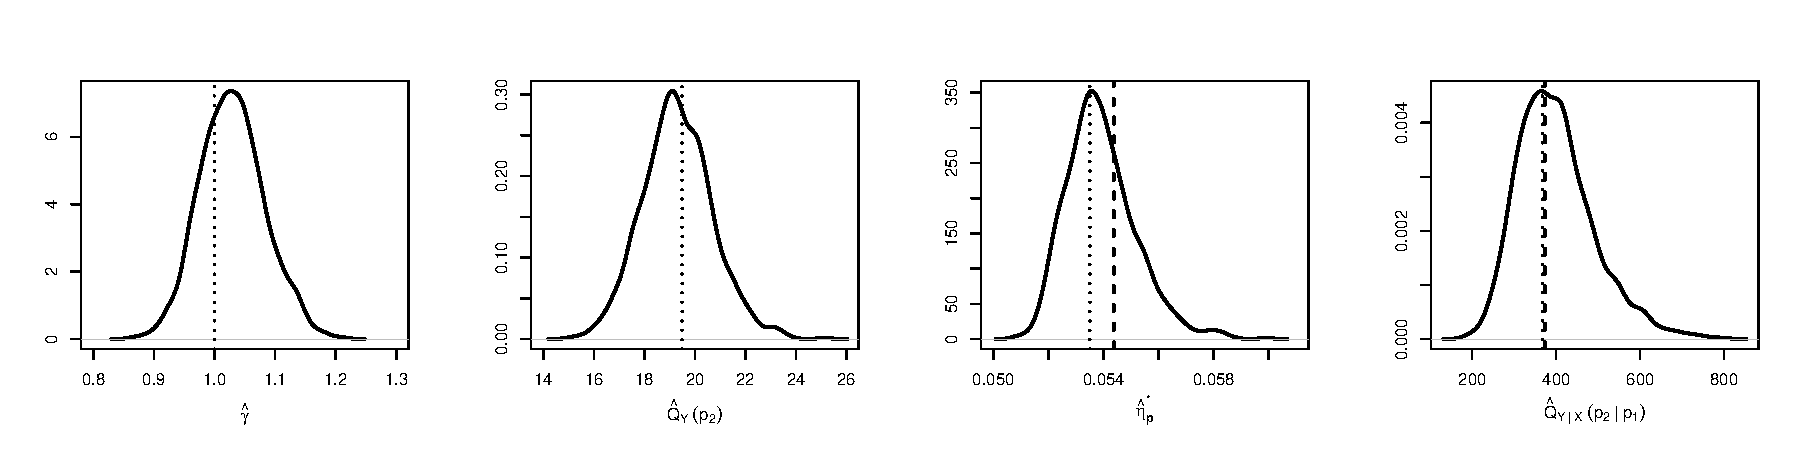
\includegraphics[width=0.98\linewidth]{log.pdf}}
    \end{figure}
    \begin{figure}[H]
    \subfigure[HR model]{
    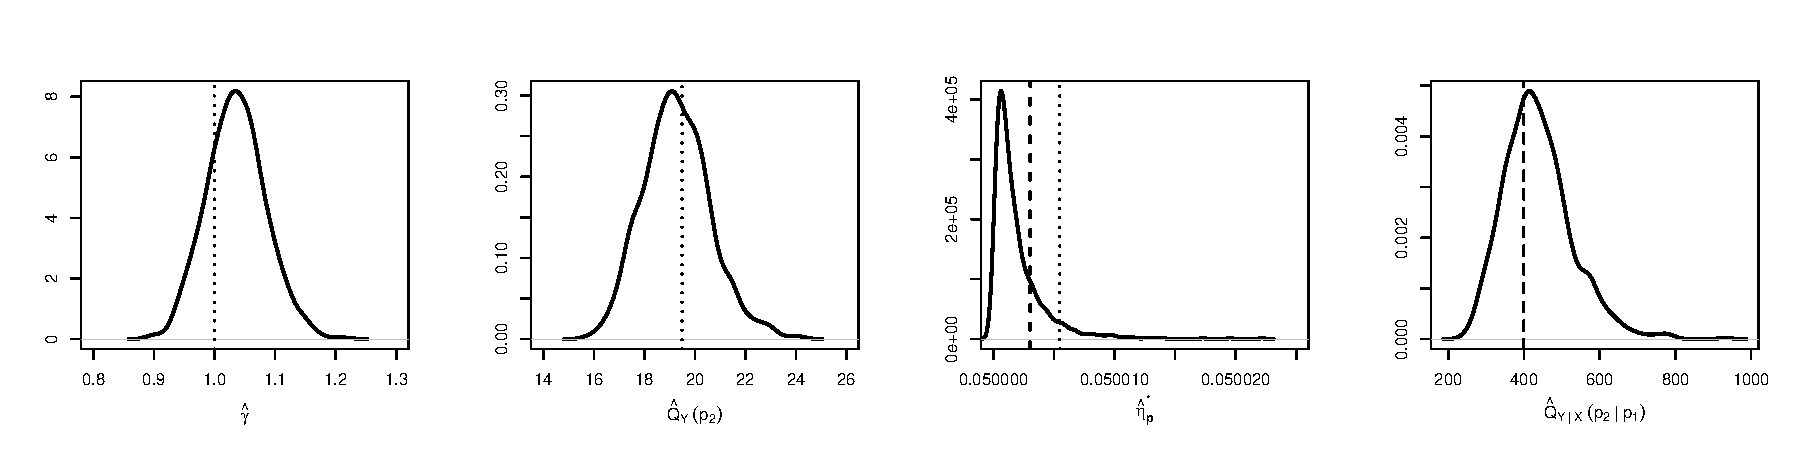
\includegraphics[width=0.98\linewidth]{hr.pdf}}
    \end{figure}
    \begin{figure}[H]
    \subfigure[Asymmetric logistic model]{
    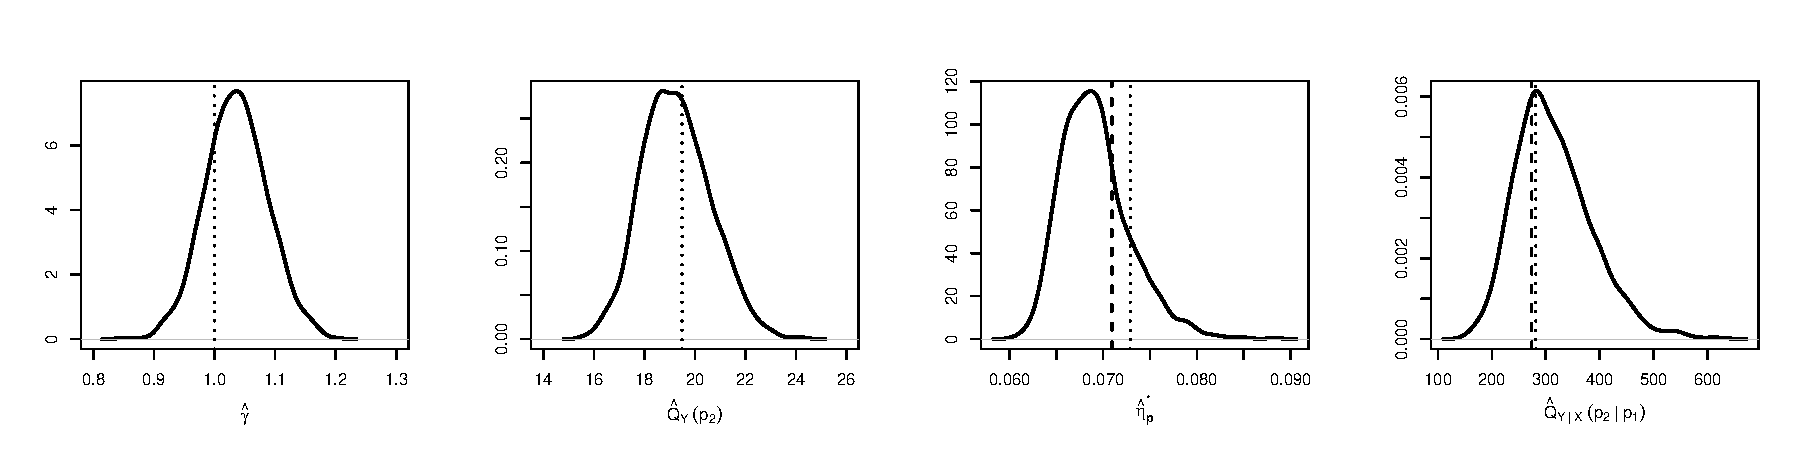
\includegraphics[width=0.98\linewidth]{alog.pdf}}
    \end{figure}
    \begin{figure}[H]
    \subfigure[Bivariate t model]{
    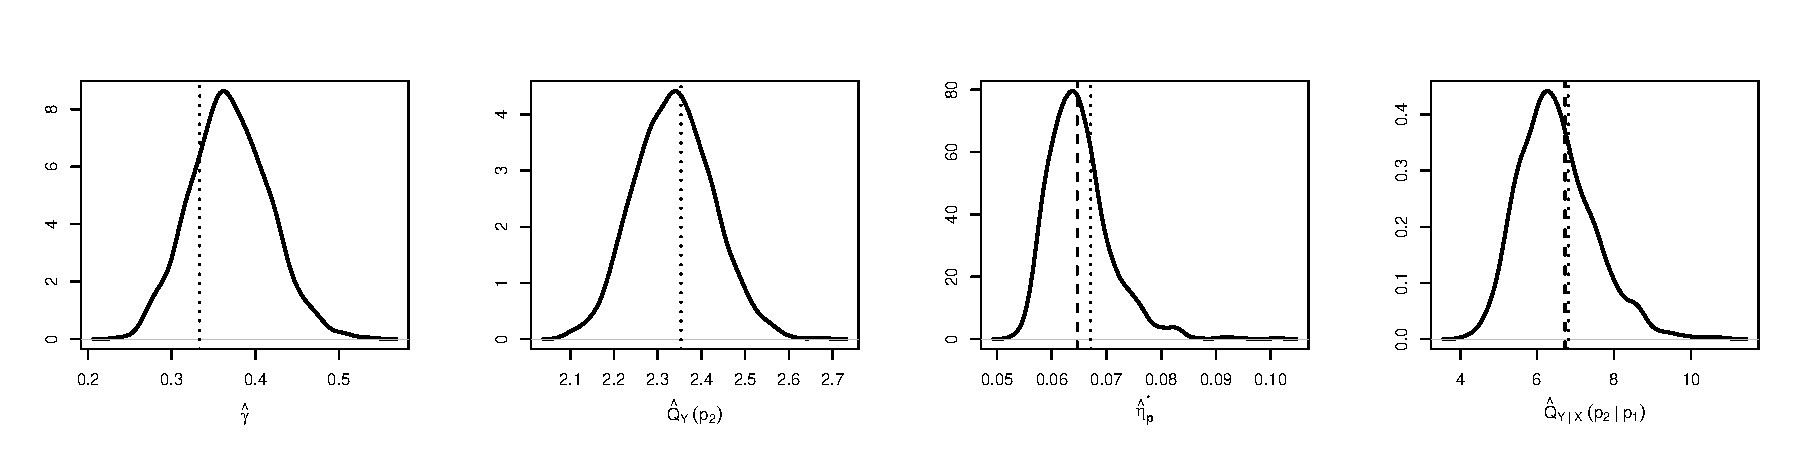
\includegraphics[width=0.98\linewidth]{t.pdf}}
  \caption{Sampling densities across 1000 replications of estimates of $\gamma$,  $Q_Y(p_2)$, $\eta_\pb^*$ and $Q_{Y|X}(p_2|p_1)$ for $p_1=p_2=0.05$ in the simulation study; see Table~\ref{sim:setup} for the simulation settings. The dotted vertical lines indicate true values of the quantities being estimated. The dashed vertical lines in the third and fourth column panels indicate the true values of $\eta_\pb$ and $Q_{Y|X}^*(p_2|p_1)$, respectively.}
  \label{sim:plot}
\end{figure}

Finally, we illustrate the asymptotic normality result of Theorem~\ref{main_theorem_asymptotic_normality}. Figure~\ref{sim:asympt_norm} displays sampling densities across 1000 replications in the simulation study of the ratio $s_n\left(\frac{\widehat{Q}_{Y|X}(p_2|p_1)}{Q_{Y|X}(p_2|p_1)}- 1\right)/\g$ and compares them with the asymptotic standard normal distribution. The sampling densities show a degree of skewness and the coverage rate is somewhat below the nominal level in the asymmetric logistic setting. There also seems to be a bias present for the bivariate t model, where the tail dependence function provides only an approximation to the underlying dependence structure in the tails. However, overall, these results suggest that asymptotic normality could be used as an approximation for inference purposes.


\begin{figure}[H]
  \centering 
    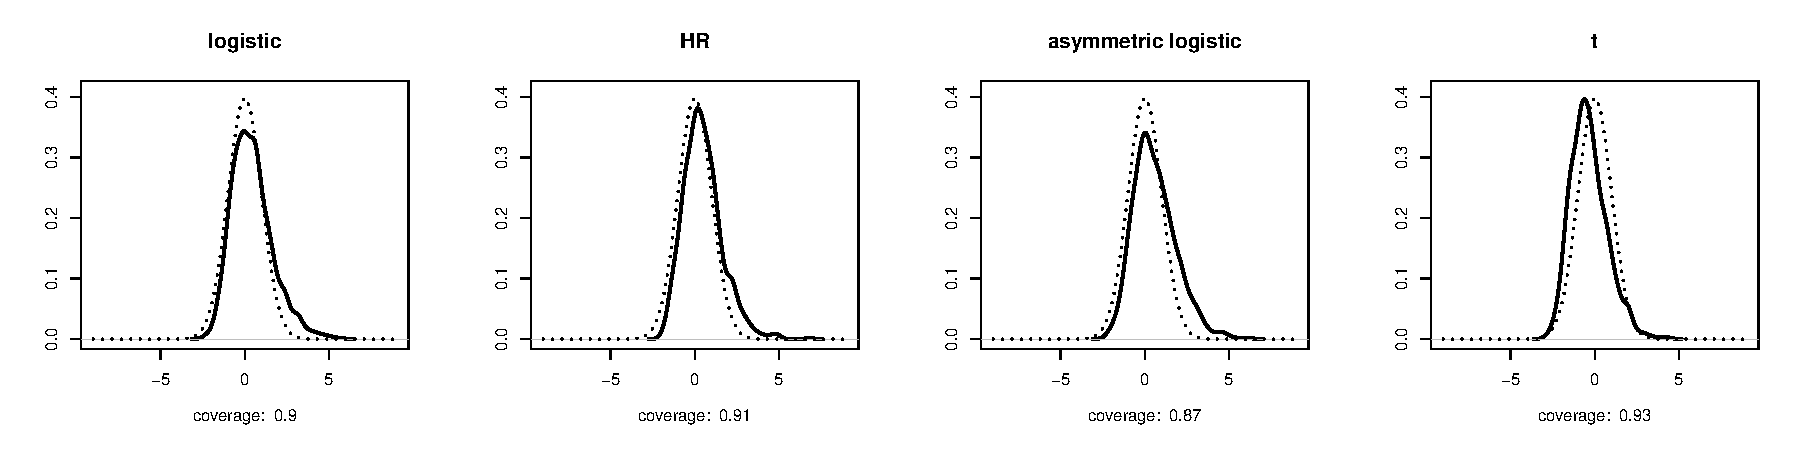
\includegraphics[width=1\linewidth]{plot_asympt_normality.pdf}
    \caption{Sampling densities across 1000 replications in the simulation study of the ratio $s_n\left(\frac{\widehat{Q}_{Y|X}(p_2|p_1)}{Q_{Y|X}(p_2|p_1)}- 1\right)/\g$ (solid lines) along with the standard normal densities (dotted lines) as an illustration of the asymptotic normality result in Theorem~\ref{main_theorem_asymptotic_normality}. The empirical coverage rates for the approximate 95\% confidence intervals for $Q_{Y|X}(p_2|p_1)$ under the four models are indicated below each plot.}
  \label{sim:asympt_norm}
    \end{figure}



\section{Application}\label{sappl}

The ECQ as defined in~\eqref{qECQ} is closely related to the concept of conditional value-at-risk (CoVaR) in finance. CoVaR at level $1-p$, denoted $\CoVaR_{Y|X}(p)$, is defined as \bql{q1}\pbb\bigl( Y\ge \CoVaR_{Y|X}(p)\mid X\ge Q_X(p)\bigr) = p,\qquad p\in(0,1),\eql
where $(1-p)$-quantile $Q_X(p)$ is commonly referred to as value-at-risk (VaR) at level $1-p$ for random variable $X$ in financial risk management literature. That is, the two functionals, ECQ and CoVaR, coincide when $p_1$ is taken to be the same as $p_2$. It should also be noted that the above definition of CoVaR is different from the original definition of CoVaR introduced by \cite{AdrianBrunnermeier2016} in that the conditioning distress event is given by the exceedence $\bigl\{X\ge Q_X(p)\bigr\}$ rather than equality $\bigl\{X= Q_X(p)\bigr\}$. This definition leads to CoVaR being dependence consistent as shown by \cite{MainikSchaanning2014}. When defining the CoVaR by conditioning on $\bigl\{X= Q_X(p)\bigr\}$, quantile regression techniques are often employed in estimation, see, e.g., \cite{AdrianBrunnermeier2016} and \cite{Leng_etal2024}. However, quantile regression cannot be used for estimating the CoVaR defined by conditioning on $\{X\ge Q_X(p)\bigr\}$ event. In the subsequent empirical study, we will use the extended definition of CoVaR based on the ECQ functional with two potentially different probability levels $p_1$ and $p_2$.



If the focal variable $Y$ is taken as the loss of a proxy for a financial system (e.g.,  a market index) and the variable in the conditioning event $X$ is the loss of a financial institution, then CoVaR can be used to assess systemic risk, the possibility that an extreme adverse event at an institution level leads to an extreme adverse event for the entire financial system. Regulators rely on measures of system risk to identify what is known as systemically important institutions, which are then subject to stricter regulatory oversight. 

In this section, we illustrate how the ECQ estimation methodology of Section~\ref{smethod} can be utilized to produce dynamic CoVaR forecasts using financial time series. In addition to assessing calibration of the resulting forecasts using the unconditional coverage test, we also conduct comparative backtests to compare forecast accuracy among different methods. The considered methods include the ones based on the proposed ECQ estimator with several parametric families for the tail dependence function as well as the one using the empirical estimator of the tail dependence function, a fully parametric method based on AR(1)-GARCH(1,1) filters for the marginals with a bivariate skew-t joint distribution for the residuals\footnote{The fully-parametric method implemented in this section is different from the method in \cite{Girardi2013}, where a bivariate DCC-GARCH model is utilized to do joint filtering. This is done in order to keep the same filtering procedure across all methods. } and the EVT-based method of \cite{NoldeZhang2018}. We refer to the last two methods as  "FP" and "EVT-NZ", respectively; both methods were extended to allow for different probability levels in the conditioning and main events to align with the ECQ definition.

We note that both the fully parametric approach using the bivariate skew-t distribution and the method of \cite{NoldeZhang2018} which is developed under the framework of multivariate regular variation implicitly assume that the residuals for both institutional and system losses exhibit heavy-tailed behaviour with the same tail index. This assumption may not always be appropriate as illustrated in Figure~\ref{fig:hill} showing estimates of the tail index for a financial institution and the S\&P~500 index. 


\begin{figure}[h]
  \centering 
    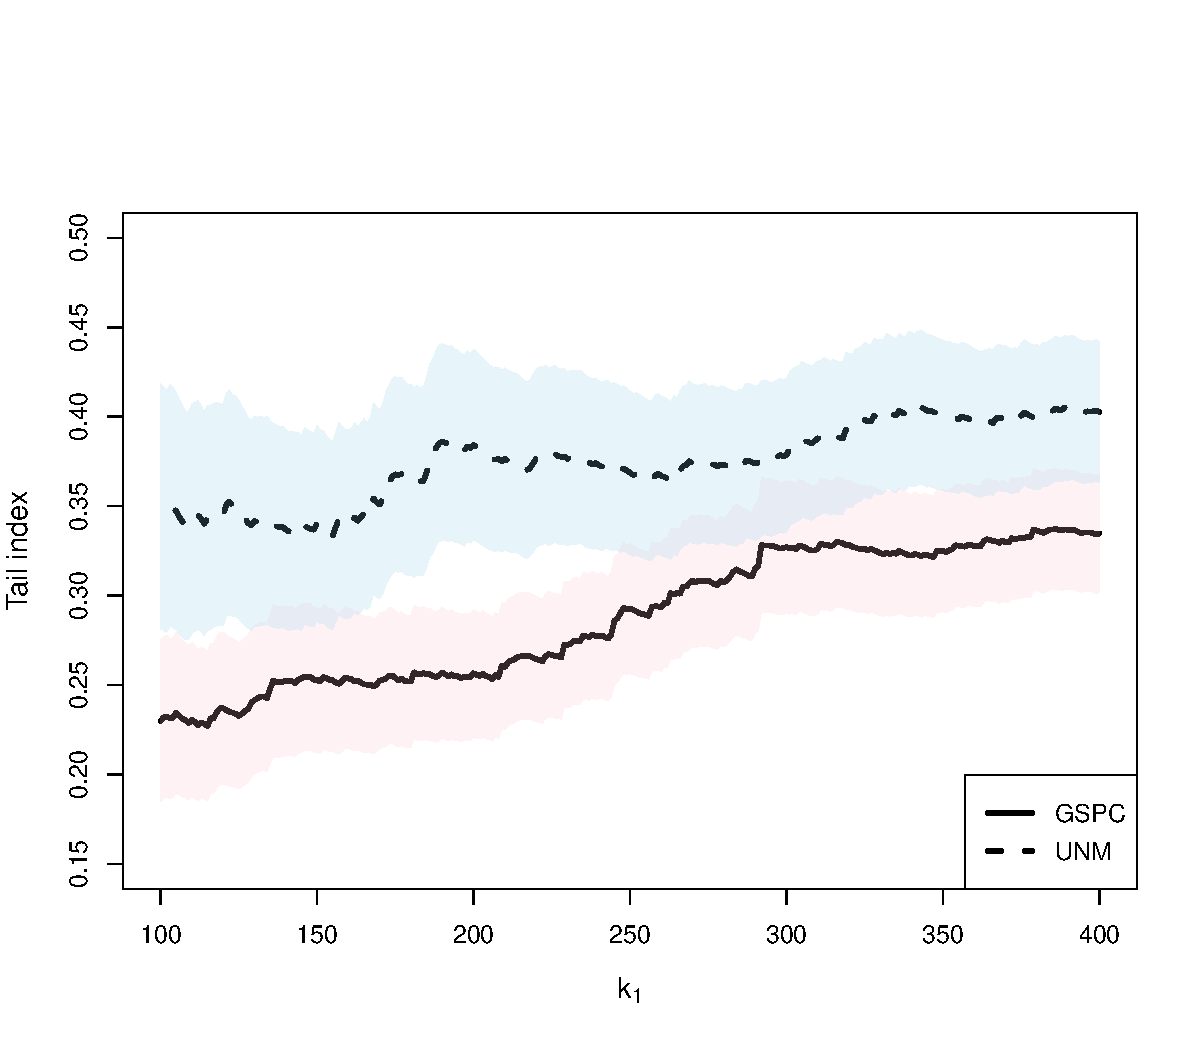
\includegraphics[width=0.5\linewidth]{hillplot_GSPC_UNM.pdf}
    \caption{Estimates of the tail index using the Hill estimator in \eqref{qHill}  as a function of~$k_1$, the number of upper order statistics used in estimation, based on the residuals from the fitted  AR(1)-GARCH(1,1) process for the daily losses of a financial institution UnumProvident Corporation (UNM) and the S\&P 500 index (GSPC) over the period 2000-2021. The shaded regions indicate asymptotic point-wise 95\% confidence bounds.}
  \label{fig:hill}
\end{figure}


\subsection{Data description}\label{data}

In our application, we consider 15 financial institutions studied in \cite{Acharya_etal2017} with a market capitalization in excess of 5 billion USD as of the end of June 2007, including Aflac Inc. (AFL), American International Group Inc. (AIG), Allstate Corp. (ALL), Bank Of America Corp. (BAC), Citigroup Inc. (C), Comerica Inc. (CMA), Humana Inc. (HUM), JPMorgan Chase \& Co. (JPM), Lincoln National Corp. (LNC), Progressive Corp. (PGR), USA Education Inc. (SLM), Travelers Companies Inc. (TRV), UnumProvident Corp. (UNM), Wells Fargo \& Co. (WFC) and Washington Mutual Inc. (WM). The S\&P 500 index (GSPC) is used as a system proxy. The sample period is from January 1, 2000 to December 30, 2021, consisting of 5535 daily closing price records for each time series. The daily losses (\%) were calculated as negative log returns. Figure~\ref{fig:time series} gives the time series plots of daily losses for one of the institutions (AFL) and the GSPC index, both displaying a typical behavior for financial time series including periods of volatility clustering such as the one during the global financial crisis of 2007--2009.

\begin{figure}[ht]
  \centering 
   \subfigure[AFL]{
    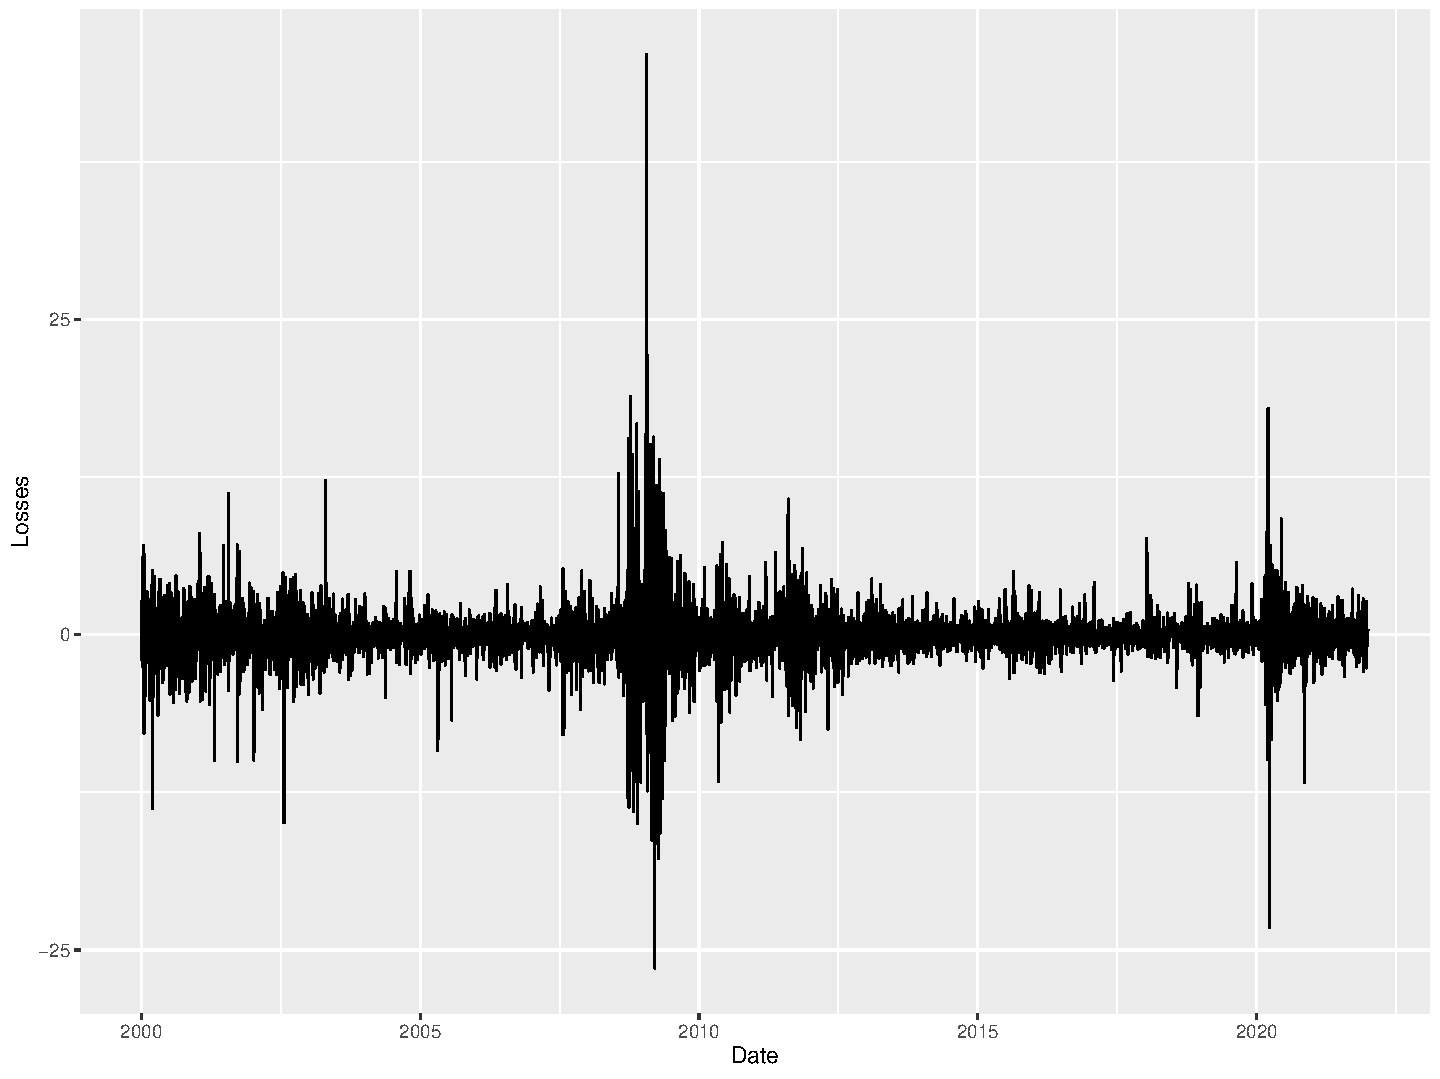
\includegraphics[width=0.4\linewidth]{ts_AFL.pdf}}
    \subfigure[S\&P 500]{
    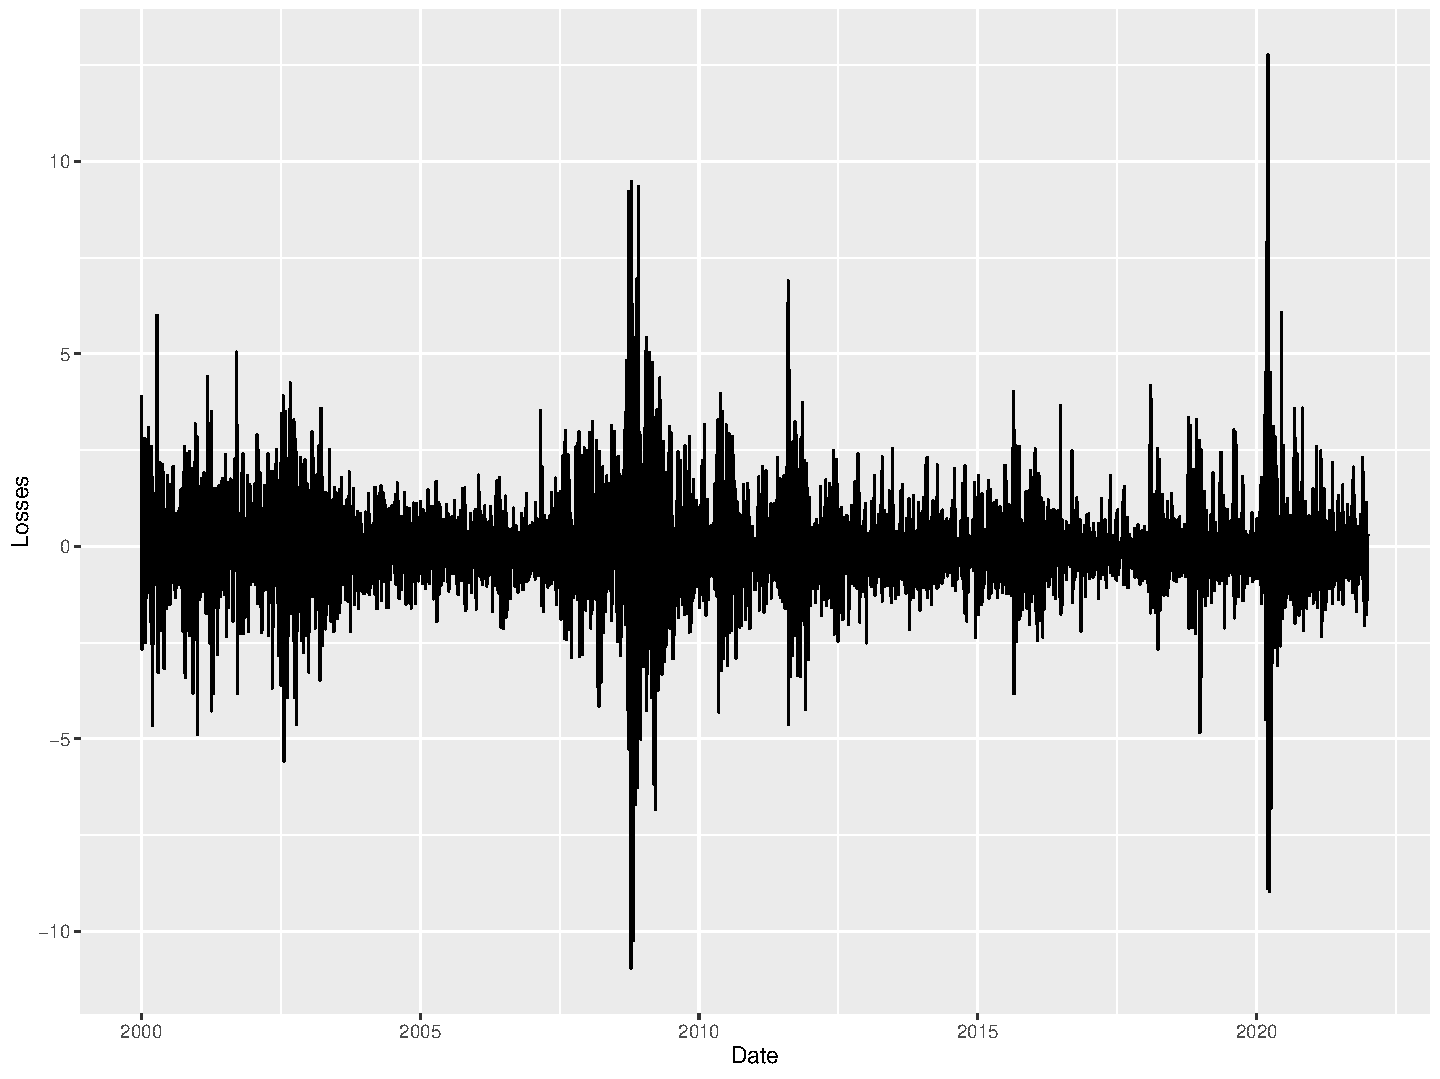
\includegraphics[width=0.4\linewidth]{ts_GSPC.pdf}}
      \caption{Time series plots of daily losses (\%) for Aflac Inc. (AFL) and the S\&P 500 index.}
  \label{fig:time series}
\end{figure}

In selection of financial institutions for the data analysis, we considered the length of their available data records as well as compliance with model assumptions for the proposed method. In addition, we chose to include institutions for which tail index estimates differed from the tail index estimate of the S\&P 500 index. Tail index estimates are summarized in Table~\ref{tab3}.


\subsection{CoVaR estimation and forecasting in the dynamic setting}\label{sappl2}

The methodology outlined in Section~\ref{smethod}, developed under the premise of i.i.d. observations, is not directly suited to produce dynamic estimates and forecasts of CoVaR for financial time series, known to possess serial dependence and display volatility clustering. One way to address this issue is by combining an ARMA-GARCH model for capturing the evolution of the conditional mean and variance of the underlying stochastic process with an EVT-based static treatment of the i.i.d. innovations; see, e.g. \cite{McNeilFrey2000}. This leads to a two-stage procedure in which first an ARMA-GARCH process is fitted to the returns (or losses) data, assuming a parametric model for innovations, followed by applying an EVT-based estimation procedure to the sample of realized innovations. 


Let $\{X_t^i\}_{t\in \nbb}$ and $\{X_t^s\}_{t\in \nbb}$ denote time series of losses for an institution (or company) and a system proxy (market index) adapted to the filtrations $\FC^i=\{\FC_t^i\}_{t\in \nbb}$ and $\FC^s=\{\FC_t^s\}_{t\in \nbb}$, respectively. To produce dynamic forecasts, we next define conditional versions of risk measures at time $t$ given information in the series up to time $t-1$.
The (conditional) VaR at confidence level $p_1\in (0,1)$ for $X_t^i$ given information on the institution's losses up to time $t-1$, denoted $\VaR^i_{t}(p_1)$,  is defined as the $(1-p_1)$-quantile of the distribution of~$X_t^i$ conditional on $\FC_{t-1}^i$:
$$\pbb\bigl(X_t^i\geq \VaR^i_{t}(p_1)\mid \FC_{t-1}^i \bigr) = p_1,$$
and $\CoVaR_{t}^{s|i}(p_2|p_1)$ is defined as the $(1-p_2)$-quantile of the conditional loss distribution given information on losses up to time $t-1$ for both the institution and the system proxy:
\begin{equation}
\label{dynamic_CoVaR}
    \pbb\bigl(X_t^s \geq \CoVaR_{t}^{s|i}(p_2|p_1) | X_t^i\geq \VaR^i_{t}(p_1);\ \FC_{t-1}^i,\   \FC_{t-1}^s\bigr) = p_2.
\end{equation}
The details of the two-stage procedure for estimating $\CoVaR_{t}^{s|i}(p_2|p_1)$ are provided in the Supplementary Material Section~\ref{sS4}, with a discussion on its theoretical validity.
\subsection{Model diagnostics}
\label{diag}
Before applying the proposed methodology to the data, we first check appropriateness of several underlying assumptions on the basis of realized innovations from the AR(1)-GARCH(1,1) filter with skew-t distributed innovations. These include independence (lack of serial dependence) and tail dependence. 


The sample autocorrelation function (acf) plots and Ljung–Box test validate the assumption of no serial correlation for most of the considered financial institutions with the exception of losses on the Travelers Companies Inc. (TRV) stock and the S\&P 500 index. In these two cases, serial dependence can be better captured using an asymmetric GARCH model, such as the exponential GARCH (eGARCH) process. However, the use of the eGARCH filter did not lead to an improvement in the out-of-sample performance of the CoVaR estimators and hence we chose to use the same (symmetric) AR(1)-GARCH(1,1) filter for all time series. 


In order to validate the assumption of tail dependence,  we estimate the upper tail dependence coefficient, $R(1,1)$ using the nonparametric estimator in~\eqref{qnpR}. The resulting estimated values are given in Table~\ref{tab3}. For all institutions, the upper tail dependence coefficient estimates are significantly greater than zero (based on a 5000-fold bootstrapping scheme), thus validating tail dependence between losses for each institution and the market index.


\begin{table}[H]
\footnotesize
\centering
\caption{Estimates of the tail index $\gamma$ for the 15 considered financial institutions and S\&P 500 index (GSPC) and of the upper tail dependence coefficient $R(1,1)$ between the institutional losses and those of the index using the nonparametric estimator in~\eqref{qnpR} with $m=200$.}
\vspace{24pt}
\begin{tabular}{c|ccccc c c c c c  c c c c c }
\hline\hline
Stock               & AFL           & AIG           & ALL           & BAC           & C       & CMA           & HUM           & JPM     \\ \hline\hline
$\hat{\gamma}$      & 0.353         & 0.349         & 0.336         & 0.308         & 0.324     & 0.335         & 0.356         & 0.307             \\
$\hat{R}(1,1)$ & 0.380 & 0.395 & 0.295 & 0.435 & 0.450 & 0.410 & 0.205  & 0.500 \\
\hline\hline
Stock        & LNC           & PGR       & SLM           & TRV           & UNM           & WFC           & WM & GSPC \\\hline\hline
$\hat{\gamma}$ & 0.314         & 0.342     & 0.330         & 0.345         & 0.369         & 0.277         & 0.359  & 0.257 \\
$\hat{R}(1,1)$  & 0.455 & 0.300 & 0.305  & 0.340  & 0.400  & 0.390 & 0.330 & $\ast$ \\
\end{tabular}
\label{tab3}
\end{table}


\subsection{Results}
\label{dynamic}
In this section, we perform a dynamic analysis to assess accuracy of one-day ahead forecasts of (extended) CoVaR at risk level $\pb = (0.02,0.05)$ for the times series described in Section~\ref{data}. The risk level is chosen so as to enable backtesting with sufficiently many observations in the marginal and joint tails. The performance of the estimator in~\eqref{qEst} under several parametric models for the tail dependence function is assessed via the unconditional coverage test with comparisons of forecast accuracy made using average quantile scores; see \cite{Banulescu_etal2020} and \cite{FisslerHoga2021} for details on backtesting of CoVaR. 

We use a rolling window of 3000 data points to estimate model parameters and produce one-day ahead CoVaR forecasts according to the two-stage procedure outlined in Section~\ref{sappl2} with further details available in the Supplementary Material Section~\ref{sS4}. The choice of the size of the estimation window balances the number of observations available for estimation (note that after conditioning on exceedances over 98\% VaR, we expect only about 60 excesses with which to estimate the conditional 95\% quantile) with the out-of-sample size of about 2500 observations available for backtesting. To reduce computational time, CoVaR and VaR estimates based on the samples of realized innovations are updated only every 50 observations. Estimation of VaR and CoVaR requires choosing suitable values for sample fractions $k_1$ and $k_2$. While it is common to take $k_2 = k_1$ and select a value with the two-step subsample bootstrap algorithm such as in \citet{Danielsson_etal2001}, we have found that this procedure leads to very low values of $k_1$ and $k_2$ for the considered datasets. As a result, in the present data analysis, we allow the two values to be different and select them separately. We first select a value of $k_1$ for the tail index estimation using the Hill plot. It suggests that $k_1 = 150$ is a good choice. We found that the performance of the proposed CoVaR estimator is more sensitive to the value of $k_2$. Thus, we adopt a procedure to select the ``best" $k_2$ by minimizing in-sample average quantile scores.

More specifically, for each rolling window of 3000 data points, we first obtain the realized innovations by applying the AR(1)-GARCH(1,1) filter. We then calculate CoVaR estimates at risk level $\pb = (0.02,0.05)$ over a sequence of $k_2$ values from 200 to 300. For each CoVaR estimate, an in-sample average quantile score can be evaluated using the classical 1-homogeneous scoring function for $(1-p_2)$-quantile: $S(r,x) = \bigl(p_2 - \ind\{x>r\}\bigr)r + \ind\{x>r\}x$ with $r$ denoting the estimate or forecast and $x$ the observation. Finally, we select $k_2$ as the one whose corresponding CoVaR estimate has the smallest average quantile score. The procedure is repeated for all the 51 windows and five parametric models. We allow $k_2$ to be different across the 51 windows and the five parametric models. A similar procedure was applied to the EVT-based method in \cite{NoldeZhang2018}, where $k_1$ and $k_2$ are involved in estimating the VaR of institutions. 

Note that when calculating the in-sample average quantile score, the VaR estimates for each institution in the conditioning event are also needed, although the proposed CoVaR estimator in~\eqref{qEst} does not involve explicit computation of the VaR estimates for institutions. Dynamic VaR estimates for institutions are also required for the purpose of out-of-sample backtesting. To keep consistency across different methods and parametric models, we take the empirical quantiles at level $1-p_1$ for each rolling window as the VaR estimates used for calculating in-sample average quantile scores and producing dynamic VaR forecasts.

Results of the unconditional coverage tests are summarized in Supplementary Material Section~\ref{uncon}. For all institutions other than LNC, the VaR estimates pass the unconditional coverage test at 5\% significance level. For most of the institutions, the CoVaR estimates under EVT-NZ method seem to be underestimated, while the fully-parametric estimates seem to be overestimated, leading to several rejections of the unconditional coverage test at level 5\% for these two methods. On the other hand, the proposed method with different models for the tail dependence function provides well-calibrated estimates of CoVaR, passing all of the unconditional coverage tests, with the exception of institution HUM modelled using the H\"usler-Reiss tail dependence function.

We would like to remark that while an analysis of the behavior of the CoVaR predictions through time is an important question, it cannot be tackled through simple means such as the Christoffersen test because the notion of transition probability over consecutive days is not applicable.

To make further comparisons across the considered methods, we summarize the average quantile scores for each CoVaR estimator in Table~\ref{ave_score}. When comparing within the proposed methodology, the asymmetric logistic and t models for the tail dependence function lead to a superior forecasting performance relative to the other three models for most of the financial institutions. Furthermore, when compared with the fully-parametric method and the EVT-based method in \cite{NoldeZhang2018}, for 12 out of 15 companies, the proposed methodology leads to a better performance in terms of accuracy of CoVaR forecasts. 


\begin{table}[ht]
\centering
\footnotesize
\caption{The average quantile scores of CoVaR forecasts at level $\pb = (0.02,0.05)$. The smallest score for each company is highlighted in bold.}
\vspace{24pt}
\begin{tabular}{ccccccc}
\hline
    & Log    & HR                & Alog            & t               & FP              & EVT-NZ         \\ \hline
AFL & 0.2767 & 0.2817           & 0.2654          & \textbf{0.2645} & 0.3087         & 0.2696          \\
AIG & 0.2667 & 0.2708           & \textbf{0.2583} & 0.2608          & 0.2903          & 0.2639          \\
ALL & 0.3016 & 0.3072           & 0.3000          & \textbf{0.2980}          & 0.3191 & 0.2992          \\
BAC & 0.2374 & 0.2404           & \textbf{0.2234} & 0.2276          & 0.2374          & 0.2406          \\
C   & 0.2412 & 0.2440           & \textbf{0.2323} & 0.2328          & 0.2396          & 0.2401          \\
CMA & 0.2562 & 0.2620           & \textbf{0.2449} & 0.2451          & 0.2626          & 0.2489          \\
HUM & \textbf{0.2409} & 0.2517 & 0.2473          & 0.2592          & 0.2781         & 0.2592          \\
JPM & 0.2325 & 0.2343           & \textbf{0.2244} & 0.2267          & 0.2351          & 0.2362          \\
LNC & 0.2319 & 0.2336           & \textbf{0.2200} & 0.2240          & 0.2385          & 0.2262          \\
PGR & 0.2673 & 0.2741           & 0.2657          & \textbf{0.2653} & 0.2740          & 0.2687          \\
SLM & 0.2366 & 0.2452           & 0.2306          & 0.2350          & 0.2516          & \textbf{0.2283} \\
TRV & 0.2786 & 0.2843           & \textbf{0.2768}          & 0.2843          & 0.2834 & 0.2826          \\
UNM & 0.2383 & 0.2419           & \textbf{0.2215} & 0.2256          & 0.2554          & 0.2337          \\
WFC & 0.2365 & 0.2394          & 0.2246          & 0.2306          & 0.2327          & \textbf{0.2224} \\
WM  & 0.2630 & 0.2749           & 0.2526          & 0.2554          & 0.2937          & \textbf{0.2502} \\ \hline
\end{tabular}
\label{ave_score}
\end{table}



Figure~\ref{figTLM} shows traffic light matrices (see, e.g., \cite{NoldeZiegel2017}) for comparative backtests at 10\% test confidence level. Comparative backtests assess  differences in average quantile scores for each pair of methods. A "proposed" method in a given row is compared with a "reference" method in a given column. A green/red square indicates that the proposed method is significantly better/worse in terms of forecasting accuracy than the reference method. Yellow squares indicate that the score differences are not statistically significant. Figure~\ref{figTLM}(a) displays the traffic light matrix for UnumProvident Corp. (UNM). It shows that the forecasting procedure using the proposed CoVaR estimator with the asymmetric logistic tail dependence function leads to a statistically significant superior forecasting performance compared to the other considered procedures. We note that this result is also supported through assessment of data properties and how they relate to various model assumptions. Figure~\ref{fig:hill}, referred to earlier in the Introduction, gives evidence of potentially different tail indices for the UNM losses and those of the S\&P 500 index, which would violate model assumptions for the fully parametric approach and the method in \cite{NoldeZhang2018}. Furthermore, carrying out a formal test in~\cite{Einmahl_etal2021} results in rejection of the null hypothesis of multivariate regular variation for these data. 

While conceptually CoVaR can be backtested in the same way as VaR, conditioning on an institution's losses being above its VaR estimate or forecast creates a practical difficulty to obtaining conclusive results when performing comparative backtesting due to substantial reduction in the size of the testing data set. For many financial institutions in our application, traffic light matrices tend to contain many yellow cells making comparisons statistically inconclusive but indicating that the proposed method is not worse than the other competing approaches. If one is interested in a method that performs best across all institutions, one possibility is to combine normalized scores. Pooling information in such a way leads to more conclusive results. Figure~\ref{figTLM}(b) shows the traffic light matrix for comparative backtests based on the normalized average scores combined across all institutions. It confirms that the proposed method with the asymmetric logistic model for the tail dependence function is significantly superior to all of the other methods in terms of its forecasting performance.


\begin{figure}[H] 
\centering
\subfigure[UNM]{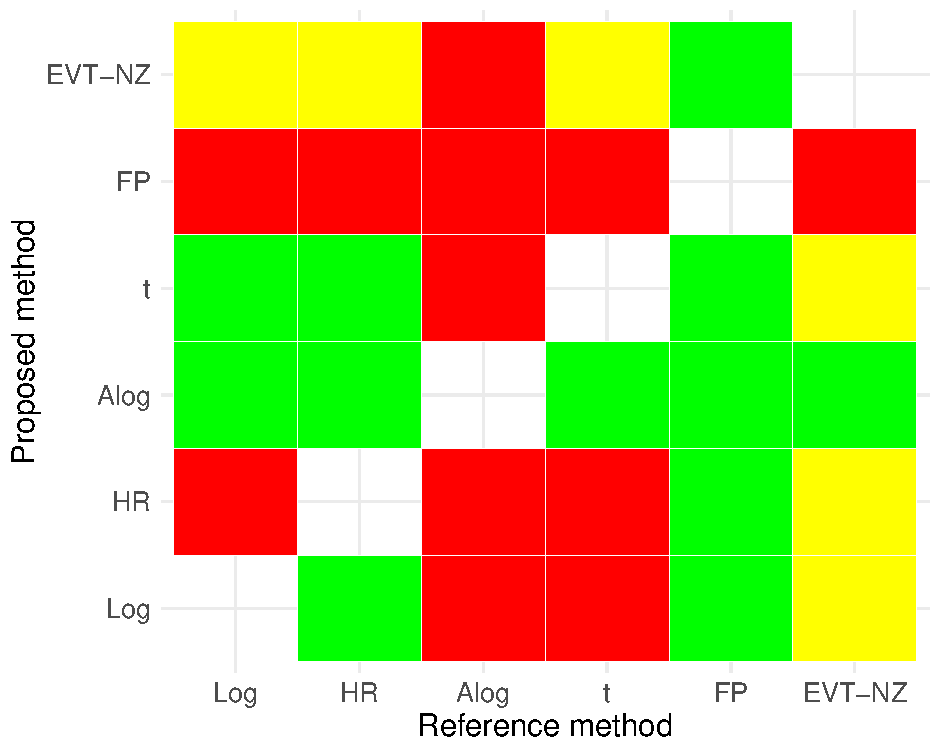
\includegraphics[width=0.4\linewidth]{TLM_UNM.pdf}}
\subfigure[All institutions]{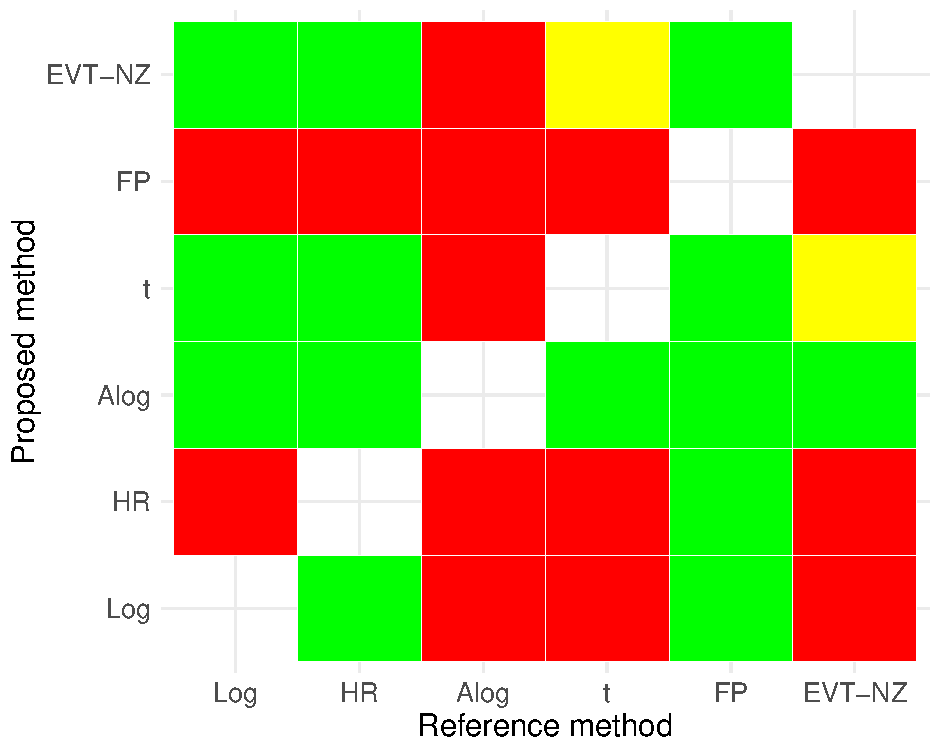
\includegraphics[width=0.4\linewidth]{TLM_outofsample.pdf}}
\caption{Traffic light matrices for comparative backtests of CoVaR one-day ahead forecasts at risk level $\pb = (0.02,0.05)$ and confidence test level of 10\%. The left panel is the result for institution UNM; the right panel is the result using the combined normalized scores across all considered institutions.}
\label{figTLM}
\end{figure}

\section{Conclusion}\label{sconc}
The paper develops an EVT-based method for estimating extreme conditional quantiles when a related variable is also extreme. Our methodology utilizes the observation that a conditional quantile can be related to the marginal quantile at an adjusted probability level. The adjustment factor is determined by the degree of (tail) dependence between the two underlying variables. A parametric modelling of the tail dependence function addresses the data sparsity issue in the joint tail regions. Expressing the ECQ as a quantile under the marginal distribution allows to then apply nonparametric extrapolation techniques in univariate tail estimation. The asymptotic theory is developed for the proposed ECQ estimator, including consistency and asymptotic normality.  Simulation studies illustrate good performance of the estimator and indicate that its bias and variance are dominated by that of the tail index estimator. Using time series data for 15 financial institutions, we find that the proposed method provides a highly competitive alternative to other existing approaches, while allowing for more flexible model assumptions.

We note that parametric modelling of the tail dependence function comes with the challenge of model selection as well as computational complexity. The latter is especially an issue when the dimension of the parameter vector of the selected model is large and the tail dependence function does not have a simple explicit form to carry through the M-estimation. Finding a more flexible yet computationally tractable way to model tail dependence may help to improve the current framework. Another limitation of the proposed methodology is that it can only be applied to situations in which the tail dependence function is non-degenerate, i.e., in the presence of tail dependence. While tail dependence is a reasonable and most relevant assumption in the context of systemic risk, in some situations, for example, in environmental applications, extending the current methodology to also include the case of tail independence will be useful. 

\section*{Supplementary Material}
In the Supplementary Material, Section~\ref{sS3} provides (upper) tail dependence functions for the five parametric models used in simulation studies and the application. Section~\ref{sup:tail_fun} contains plots of tail dependence function $R(1,\eta)$ as a function of $\eta$ under several tail dependence models. Section~\ref{sS4} details the two-stage procedure for producing dynamic CoVaR forecasts. Section~\ref{uncon} presents results of the unconditional coverage tests in the application. Section~\ref{sup:Sim_Model_Misspecification} summarizes results of a simulation study under model misspecification.


\section*{Acknowledgements} We are grateful to the three reviewers for providing constructive feedback and valuable comments. N. Nolde and M. Zhou acknowledge financial support of the UBC-Scotiabank Risk Analytics Initiative and Natural Sciences and Engineering Research Council of Canada. 


%%%%%%%%%%%%%%%%%%%%%%%%%%%%%%%%%%%%%%%%%%%%%%%%%
\bibliographystyle{plainnat} 

\begin{thebibliography}{29}
\providecommand{\natexlab}[1]{#1}
\providecommand{\url}[1]{\texttt{#1}}
\expandafter\ifx\csname urlstyle\endcsname\relax
  \providecommand{\doi}[1]{doi: #1}\else
  \providecommand{\doi}{doi: \begingroup \urlstyle{rm}\Url}\fi

\bibitem[Acharya et~al.(2017)Achaya, Pedersen, Philippon, and Richardson]{Acharya_etal2017}
V.V. Acharya, L.H. Pedersen, T.~Philippon, M.~Richardson.
\newblock {Measuring systemic risk}.
\newblock \emph{The Review of Financial Studies}, 30:2--47, 2017.


\bibitem[Adrian and Brunnermeier(2016)]{AdrianBrunnermeier2016}
T.~Adrian and M.K. Brunnermeier.
\newblock {CoVaR}.
\newblock \emph{American Economic Review}, 106:1705--1741, 2016.


\bibitem[Banulescu-Radu et~al.(2020)Banulescu-Radu, Hurlin, Leymarie, and
  Scaillet]{Banulescu_etal2020}
D.~Banulescu-Radu, C.~Hurlin, J.~Leymarie, and O.~Scaillet.
\newblock Backtesting marginal expected shortfall and related systemic risk
  measures.
\newblock \emph{Management Science}, 67:\penalty0 5730--5754, 2020.


\bibitem[Cai et~al.(2014)]{Cai2014}
J.~Cai, J.~Einmahl, L.~de Haan and C. Zhou.
\newblock Estimation of the marginal expected shortfall: the mean when a related variable is extreme.
\newblock \emph{Journal of the Royal Statistical Society: Series B},
  77:\penalty0 417--442, 2014.


\bibitem[Coles and Tawn(1991)]{ColesTawn1991}
S.G. Coles and J.A. Tawn.
\newblock Modelling extreme multivariate events.
\newblock \emph{Journal of the Royal Statistical Society: Series B},
  53:\penalty0 377--392, 1991.

\bibitem[Danielsson et~al.(2001)Danielsson, de~Haan, Peng, and
  de~Vries]{Danielsson_etal2001}
J.~Danielsson, L.~de~Haan, L.~Peng, and C.G. de~Vries.
\newblock Using a bootstrap method to choose the sample fraction in tail index
  estimation.
\newblock \emph{Journal of Multivariate Analysis}, 76:\penalty0 226--248, 2001.

\bibitem[de~Haan and Ferreira(2006)]{dHF2006}
L.~de~Haan and A.~Ferreira.
\newblock \emph{Extreme Value Theory: An Introduction}.
\newblock Springer Science \& Business Media, 2006.

\bibitem[Einmahl et~al.(2008)Einmahl, Krajina, and Segers]{Einmahl_etal2008}
J.H. Einmahl, A.~Krajina, and J.~Segers.
\newblock A method of moments estimator of tail dependence.
\newblock \emph{Bernoulli}, 14:\penalty0 1003--1026, 2008.

\bibitem[Einmahl et~al.(2012)Einmahl, Krajina, and Segers]{Einmahl_etal2012}
J.H. Einmahl, A.~Krajina, and J.~Segers.
\newblock An {M}-estimator for tail dependence in arbitrary dimensions.
\newblock \emph{The Annals of Statistics}, 40:\penalty0 1764--1793, 2012.

\bibitem[Einmahl et~al.(2018)Einmahl, Kiriliouk, and Segers]{Einmahl_etal2018}
J.H. Einmahl, A.~Kiriliouk, and J.~Segers.
\newblock A continuous updating weighted least squares estimator of tail dependence in high dimensions.
\newblock \emph{Extremes}, 21:\penalty0 205--233, 2018.





\bibitem[Einmahl et~al.(2021)Einmahl, Yang and Zhou]{Einmahl_etal2021}
J.H. Einmahl, F.~Yang, and C.~Zhou.
\newblock Testing the multivariate regular variation model.
\newblock \emph{Journal of Business \& Economic Statistics}, 39:\penalty0 907--919, 2021.


\bibitem[Fissler and Hoga(2021)]{FisslerHoga2021}
T.~Fissler and Y.~Hoga.
\newblock Backtesting systemic risk forecasts using multi-objective
  elicitability.
\newblock \emph{arXiv preprint arXiv:2104.10673}, 2021.



\bibitem[Girardi and Erg{\"u}n(2013)]{Girardi2013}
G.~Girardi and A.T. Erg{\"u}n.
\newblock Systemic risk measurement: Multivariate {GARCH} estimation of
  {CoVaR}.
\newblock \emph{Journal of Banking \& Finance}, 37:\penalty0 3169--3180, 2013.

\bibitem[Gnedenko(1943)]{Gnedenko1943}
B.V. Gnedenko.
\newblock Sur la distribution limit\'e du terme d'une s\'erie al\'eatoire.
\newblock \emph{Ann. Math.}, 44:\penalty0 423--453, 1943.

\bibitem[Hill(1975)]{Hill1975}
B.M. Hill.
\newblock A simple general approach to inference about the tail of a
  distribution.
\newblock \emph{The Annals of Statistics}, 3:1163--1174, 1975.


\bibitem[Hoga(2019)]{Hoga2019}
Y. Hoga.
\newblock Confidence intervals for conditional tail risk measures in ARMA--GARCH models.
\newblock \emph{Journal of Business \& Economic Statistics}, 37(4): 613--624, 2019.



\bibitem[H{\"u}sler and Reiss(1989)]{HuslerReiss1989}
J.~H{\"u}sler and R.D. Reiss.
\newblock Maxima of normal random vectors: between independence and complete
  dependence.
\newblock \emph{Statistics \& Probability Letters}, 7:\penalty0 283--286, 1989.

\bibitem[Joe et~al.(1992)Joe, Smith, and Weissman]{Joe_etal1992}
H.~Joe, R.L. Smith, and I.~Weissman.
\newblock Bivariate threshold methods for extremes.
\newblock \emph{Journal of the Royal Statistical Society: Series B},
  54:\penalty0 171--183, 1992.

\bibitem[Joe(1997)]{Joe1997}
H. Joe.
\newblock \emph{Multivariate Models And Multivariate Dependence Concepts}.
\newblock Chapman and Hall/CRC, 1997.

\bibitem[Ledford and Tawn(1996)]{LedfordTawn1996}
A.W. Ledford and J.A. Tawn.
\newblock Statistics for near independence in multivariate extreme values.
\newblock \emph{Biometrika}, 83:\penalty0 169--187, 1996.


\bibitem[Leng et al. (2024)]{Leng_etal2024}
X. Leng, Y. He,  Y. Hou and L. Peng. 
\newblock Asymptotics of CoVaR Inference In Two-Quantile-Regression.
\newblock \emph{Available at SSRN: \href{https://ssrn.com/abstract=4816475}{https://ssrn.com/abstract=4816475} }, 2024.



\bibitem[Mainik and Schaanning(2014)]{MainikSchaanning2014}
G.~Mainik and E.~Schaanning.
\newblock On dependence consistency of {CoVaR} and some other systemic risk
  measures.
\newblock \emph{Statistics \& Risk Modeling}, 31:\penalty0 49--77, 2014.

\bibitem[McNeil and Frey(2000)]{McNeilFrey2000}
A.J. McNeil and R.~Frey.
\newblock Estimation of tail-related risk measures for heteroscedastic
  financial time series: an extreme value approach.
\newblock \emph{Journal of Empirical Finance}, 7:\penalty0 271--300, 2000.

\bibitem[McNeil et~al.(2005)McNeil, Frey, and Embrechts]{QRM}
A.J. McNeil, R.~Frey, and P.~Embrechts.
\newblock \emph{Quantitative Risk Management: Concepts, Techniques And Tools.}
\newblock Princeton University Press, Princeton, 2005.

\bibitem[Nolde and Zhang(2020)]{NoldeZhang2018}
N.~Nolde and J.~Zhang.
\newblock Conditional extremes in asymmetric financial markets.
\newblock \emph{Journal of Business \& Economic Statistics}, 38: 201--213, 2020.

\bibitem[Nolde and Ziegel(2017)]{NoldeZiegel2017}
N.~Nolde and J.~Ziegel.
\newblock Elicitability and backtesting: Perspectives for banking regulation.
\newblock \emph{The Annals of Applied Statistics}, 11:\penalty0 1833--1874,
  2017.

\bibitem[Resnick(1987)]{Resnick1987}
S.I. Resnick.
\newblock \emph{Extreme Values, Regular Variation and Point Processes}.
\newblock Springer, 1987.

\bibitem[Smith(1990)]{Smith1990}
R.L. Smith.
\newblock Extreme value theory.
\newblock \emph{Handbook of Applicable Mathematics}, 7:\penalty0 437--471,
  1990.

\bibitem[Smith(1994)]{Smith1994}
R.L. Smith.
\newblock Multivariate threshold methods.
\newblock In \emph{Extreme Value Theory and Applications}, pages 225--248.
  Springer, 1994.

\bibitem[Weissman(1978)]{Weissman1978}
I.~Weissman.
\newblock Estimation of parameters and large quantiles based on the $k$ largest
  observations.
\newblock \emph{Journal of the American Statistical Association}, 73:\penalty0
  812--815, 1978.

\end{thebibliography}
%%%%%%%%%%%%%%%%%%%%%%%%%%%%%%%%%%%%%%%%%%%%%%%%%%%%%%


\clearpage
\appendix
\def\thesection{Appendix \Alph{section}}
\def\thetheorem{\Alph{section}.\arabic{theorem}}
\setcounter{equation}{0}
\renewcommand{\theequation}{A.\arabic{equation}}

\setcounter{page}{1}

%\begin{center}
%    {\LARGE Tail risk in the tail: Estimating high quantiles when a related variable is extreme\\
%  \bf Appendix\\
%  }
%\end{center}
%\change{CZ: I adapted the proofs for the general CoVaRs. The cross reference is not yet correct.}

\section{Proof of Theorems \ref{main theorem}}
\label{appen_proofA}
Recall the definition of $\h_\pb$:
$$\h_\pb = \dfrac{\pbb\bigl(Y\ge Q_{Y|X}(p_2|p_1)\bigr)}{\pbb\bigl(Y\ge Q_{Y|X}(p_2|p_1)\mid X\ge Q_X(p_1)\bigr)}\in(0,1],\qquad p_1,p_2\in(0,1).$$
We can then rewrite the ratio $\frac{\widehat{Q}_{Y|X}(p_2|p_1)}{Q_{Y|X}(p_2|p_1)}$ as 
\begin{align*}
    \frac{\widehat{Q}_{Y|X}(p_2|p_1)}{Q_{Y|X}(p_2|p_1)} &=\frac{\left(\h_\pb^*\right)^{-\hat\gamma}\widehat{Q}_Y(p_2)}{Q_Y(p_2\h_\pb)}\\
    &=\left(\frac{\h_\pb^*}{\h_\pb}\right)^{-\hat\gamma}\times \h_\pb^{\gamma-\hat\gamma
    } \times \frac{\widehat{Q}_Y(p_2)}{Q_Y(p_2)} \times\frac{\left(\h_\pb\right)^{-\gamma}Q_Y(p_2)}{Q_Y(p_2\h_\pb)} \\
    &=:I_1\times I_2\times I_3\times I_4.
\end{align*}
The theorem is proved by showing that, as $n\to\infty$, $I_j\top1$ for $j=1,2,3,4$. 

Before handling these four terms, the following two lemmas provide some preliminary results regarding the quantities $\h_\pb$ and $\h^*_\pb$ as well as the estimator $\hat\h^*_\pb$.

\begin{lemma} \label{lem:eta* and hat eta*}
    Under the same conditions as in Theorem \ref{main theorem}, we have that, as $n\to\infty$,
$$\frac{p_1}{\h^*_\pb}\to R_2(1,0;\thb_0) \text{\ and \ }\frac{p_1}{\hat\h^*_\pb}\top R_2(1,0;\thb_0).$$
\end{lemma}
\begin{lemma} \label{lem:eta and eta*}
    Under the same conditions as in Theorem \ref{main theorem}, we have, as $n\to\infty$,
    $$\frac{\h_\pb}{\h^*_\pb}\to1.$$
\end{lemma}
\begin{proof}[Proof of Lemma \ref{lem:eta* and hat eta*}]
In order to prove the limit relation regarding $\h^*_\pb$, we first show that as $n\to\infty$, $\h^*_\pb\to 0$. If otherwise, then there exists a subsequence of integers, $\{n_l\}$ such that $\h^*_{\pb(n_l)}\to c'>0$ as $l\to\infty$. W.l.o.g., we still use the notation $n$ instead of $n_l$. Then, as $n\to\infty$, $R\left(1,\h^*_\pb\frac{p_2}{p_1};\thb_0\right)\to R\left(1,\frac{c'}{c};\thb_0\right)>0$ which follows from $\frac{p_1}{p_2}\to c$ in \ref{con:p} and the fact that $R(1,y;\thb_0)$ is a non-decreasing function in $y$. However, this contradicts with $R\left(1,\h^*_\pb\frac{p_2}{p_1};\thb_0\right)=p_2\to 0$ as $n\to\infty$. Hence, we conclude that $\h^*_\pb\to 0$ as $n\to\infty$.

Using the mean value theorem, we have that there exists a series of constants $\xi_n\in[0, \h^*_\pb\frac{p_2}{p_1}]$ such that
$$
p_2=R\left(1,\h^*_\pb\frac{p_2}{p_1};\thb_0\right)=R(1,0;\thb_0)+\h^*_\pb\frac{p_2}{p_1} R_2(1,\xi_n;\thb_0)=\h^*_\pb\frac{p_2}{p_1} R_2(1,\xi_n;\thb_0).
$$
Hence we get that, as $n\to\infty$,
$$\frac{p_1}{\h^*_\pb}=R_2(1,\xi_n;\thb_0)\to R_2(1,0;\thb_0).$$
Here in the last step, we use the fact that $\xi_n\to 0$ as $n\to\infty$ and $R_2(x,y;\thb_0)$ is a continuous function at $(1,0;\thb_0)$.

The proof for the limit relation regarding $\hat\h^*_\pb$ follows similarly by replacing $\thb_0$ with $\hat\thb$ and using the fact that $\hat\thb\top\thb_0$ as $n\to\infty$. We therefore omit the details.
\end{proof}


\begin{proof}[Proof of Lemma \ref{lem:eta and eta*}]
    We first show that, as $n\to\infty$, $\h_\pb\to 0$. If assuming otherwise, there exists a subsequence of integers, $\{n_l\}$ such that $\h_{\pb(n_l)}\to c>0$ as $l\to\infty$. W.l.o.g., we still use the notation $n$ instead of $n_l$. Recall the definition of $\h_\pb$:
    $$\frac{\pbb(X>Q_X(p_1),Y>Q_Y(p_2\h_\pb))}{p_1}=p_2.$$
    By taking $n\to\infty$ on both sides of this equation, and using the assumption $\h_\pb\to c'>0$ together with $\frac{p_1}{p_2}\to c$ as $n\to\infty$, we get that
    $R(1,\frac{c'}{c};\thb_0)=0$, which contradicts \ref{con:R2} and the fact that $R(1,y;\thb_0)$ is a non-decreasing function in $y$. Hence, we conclude that, as $n\to\infty$, $\h_\pb\to 0$.
    
    
Next we show, by contradiction, that 
$$\limsup_{n\to\infty}\frac{\h_\pb}{\h^*_\pb}\leq 1.$$
If assuming otherwise, there exists a subsequence of $n$, $\{n_l\}_{l=1}^\infty$ such that as $l\to\infty$, $n_l\to\infty$ and
$$\frac{\h_{\pb(n_l)}}{\h^*_{\pb(n_l)}}\to c'>1.$$
W.l.o.g., we still use the notation $n$ for the subsequence, and omit it by writing $\pb=\pb(n)$. Therefore, for any $1<\tilde c<c$, there exists $n_0=n_0(\tilde c)$ such that for $n>n_0$, $\frac{\h_\pb}{\h^*_\pb}>\tilde c.$

Note that $\h_\pb>\tilde c \h^*_\pb>\h^*_\pb$. By the mean value theorem, we get that for each $n$, there exists $\xi_n\in\left(\frac{p_2}{p_1}\h^*_\pb,\frac{p_2}{p_1}\h_\pb\right)$ such that 
\begin{equation} \label{eq:compare eta and eta*}
R\left(1,\frac{p_2}{p_1}\h_\pb;\thb_0\right) -R\left(1,\frac{p_2}{p_1}\h^*_\pb;\thb_0\right) =R_2(1,\xi_n;\thb_0)\frac{p_2}{p_1}(\h_\pb-\h^*_\pb).
\end{equation}
As $n\to\infty$, since both $\h^*_\pb\to 0$ and $\h_\pb\to 0$ hold, we get $\xi_n\to 0$. Further note that $\h_\pb-\h^*_\pb>(\tilde c-1)\h^*_\pb$. By applying Lemma \ref{lem:eta* and hat eta*} and the continuity of $R_2(x,y;\thb)$ at $(1,0;\thb_0)$, we get that 
\begin{align*}
\liminf_{n\to\infty}\frac{R\left(1,\frac{p_2}{p_1}\h_\pb;\thb_0\right) -p_2}{p_1}&=\liminf_{n\to\infty}\frac{R\left(1,\frac{p_2}{p_1}\h_\pb;\thb_0\right) -R\left(1,\h^*_\pb\frac{p_2}{p_1};\thb_0\right)}{p_1}\\
&=\liminf_{n\to\infty}\frac{R\left(1,\frac{p_2}{p_1}\h_\pb;\thb_0\right) -R\left(1,\frac{p_2}{p_1}\h^*_\pb;\thb_0\right)}{\h^*_\pb}\times\frac{\h^*_\pb}{p_1}\\
&\geq R_2(1,0;\thb_0)\frac{\tilde c-1}{c}\times \frac{1}{R_2(1,0;\thb_0)}=\frac{\tilde c-1}{c}>0.
\end{align*}
Since \ref{con:soc for R} holds with $\tilde\rho>1$, we get that
\begin{align*}
    \lim_{n\to\infty}\frac{R\left(1,\frac{p_2}{p_1}\h_\pb;\thb_0\right) -p_2}{p_1}&=\lim_{n\to\infty}\frac{1}{p_1}\left(R\left(1,\frac{p_2}{p_1}\h_\pb;\thb_0\right)-\frac{1}{p_1}\pbb\left(X>Q_X(p_1),Y>Q_Y\left(p_1\cdot\frac{p_2}{p_1}\h_\pb\right)\right)\right)\\
    &=0.  
\end{align*}
The two limit relations contradict each other. Therefore, we conclude that $$\limsup_{n\to\infty}\frac{\h_\pb}{\h^*_\pb}\leq 1.$$
Similarly, one can show a lower bound for $\frac{\h_\pb}{\h^*_\pb}$, which completes the proof of the lemma.
\end{proof}

Now we turn to prove the main theorem by handling the four terms $I_j$, $j=1,2,3,4$.

Firstly, we handle $I_1$. Following the asymptotic property of the Hill estimator (e.g., Theorem 3.2.5 in \cite{dHF2006_sup}), \ref{con:soc} and \ref{con:k} for $k_1$ imply that as $n\to\infty$, 
\begin{equation}\label{eq:asymptotic Hill}
    \sqrt{k_1}(\hat\gamma-\gamma)\stackrel{d}{\to} \NC\left(\frac{\lambda_1}{1-\rho},\gamma^2\right),
\end{equation}
which implies that
$\hat\gamma\top \gamma$. Together with Lemma \ref{lem:eta and eta*} and Lemma \ref{lem:eta* and hat eta*}, we conclude that $I_1\top 1$ as $n\to\infty$.

Secondly, we handle $I_2$. Given the limit relation in \eqref{eq:asymptotic Hill}, we only need to show that $\log (\h_\pb)/\sqrt{k_1}\to 0$ as $n\to\infty$. From Lemma \ref{lem:eta* and hat eta*} and Lemma \ref{lem:eta and eta*}, we get that $\h_\pb/p_1\to 1/R_2(1,0,\thb_0)$ as $n\to\infty$. Together with the limit relation regarding $k_1$ in \ref{con:k}, we get that $I_2\top 1$ as $n\to\infty$.

The term $I_3$ is handled by the asymptotic property of the high quantile estimator; see, e.g. Theorem 4.3.8 in \cite{dHF2006_sup}. More specifically, under \ref{con:soc}, \ref{con:k} and \ref{con:p}, the high quantile estimator in Section~\ref{method:est} has the following asymptotic property: as $n\to\infty$,
$$ \min\left(\sqrt{k_2},\frac{\sqrt{k_1}}{\log (k_2/np_2)}\right)\left(\frac{\widehat{Q}_Y(p_2)}{Q_Y(p_2)}-1\right)=O_P(1). $$
The result follows from the proof of Theorem 4.3.8 in \cite{dHF2006_sup} with some proper adaptations. A direct consequence is that $I_3\top1$ as $n\to\infty$.

Finally, we handle the deterministic term $I_4$. Notice that $Q_Y(p_2)=U_Y(1/p_2)$ and $Q_Y(p_2\h_\pb)=U_Y(1/(p_2\h_\pb))$. By applying \ref{con:soc} with $t=1/p$ and $x=1/\h_\pb$, we get that
$$\lim_{n\to\infty}\frac{\frac{Q_Y(p_2\h_\pb)}{Q_Y(p_2)}\h_\pb^\gamma-1}{A(1/p)}=-\frac{1}{\rho}.$$
As $n\to\infty$, since $A(1/p)\to0$ we get that $I_4\to 1$.
\qed

%\change{CZ: Here is the old proof. We should delete it.}
%\begin{proof}[Proof of Theorem \ref{main theorem: general CoVaR}]
%    Write
%    \begin{align*}
%        \frac{\widehat{Q}_{Y|X}(p_2|p_1)}{Q_{Y|X}(p_2|p_1)} &=\left(\frac{\hat\eta_\pb^*}{\eta_\pb}\right)^{-\hat\gamma}\times \eta_\pb^{\gamma-\hat\gamma
%        } \times \frac{\widehat{Q}_Y(p_2)}{Q_Y(p_2)} \times\frac{\left(\eta_\pb\right)^{-\gamma}Q_Y(p_2)}{Q_Y(p_2\eta_\pb)} \\
%        &=:I_1\times I_2\times I_3\times I_4.
%    \end{align*}
%    
%    The main difference lies in verifying that  Lemma \ref{lem:eta* and hat eta*} and \ref{lem:eta and eta*} hold with replacing $\eta^*_p$, $\hat\eta^*_p$ and $p$ by $\eta^*_\pb$, $\hat\eta^*_\pb$ and $p_1$, respectively. That is, as $n\to\infty$,
%    $$\frac{p_1}{\eta^*_\pb}\to R_2(1,0;\thb_0) \text{\ and \ } \frac{p_1}{\hat\eta^*_\pb}\to R_2(1,0;\thb_0); \:\:\:\frac{\eta_\pb}{\eta^*_\pb}\to 1.$$
%    These results guarantees that both $I_1\top 1$ and $I_2\top 1$ as $n\to\infty$. Together with the consistency results for $I_3$ and $I_4$, the theorem is proved.
%\end{proof}

%%%%
\section{Proof of Theorems \ref{main_theorem_asymptotic_normality} } \label{appen_proofB}
%    \change{We should change the title. Maybe
%         Theorem \ref{main_theorem_asymptotic_normality} refers to the general case now? If so, we can remove Theorem \ref{main_theorem_asymptotic_normality: general CoVaR} from the title of the section.}

    Similar to the proof of consistency, using the notation $Q_Y(p)=U_Y(1/p)$, we  write the ratio $\frac{\widehat{Q}_{Y|X}(p_2|p_1)}{Q_{Y|X}(p_2|p_1)}$ as 
    \begin{align*}
        \frac{\widehat{Q}_{Y|X}(p_2|p_1)}{Q_{Y|X}(p_2|p_1)} &=\frac{\left(\hat\h_\pb^*\right)^{-\hat\gamma}\widehat{Q}_Y(p_2)}{Q_Y(p_2\h_\pb)}\\
        &=\left(\frac{\hat\h_\pb^*}{\h_\pb}\right)^{-\hat\gamma}\times \h_\pb^{\gamma-\hat\gamma
        } \times \frac{\widehat{Q}_Y(p_2)}{Q_Y(p_2)} \times\frac{\left(\h_\pb\right)^{-\gamma}Q_Y(p_2)}{Q_Y(p_2\h_\pb)} \\
        &=\left(\frac{\hat\h_\pb^*}{\h_\pb}\right)^{-\hat\gamma}\times \h_\pb^{\gamma-\hat\gamma
        } \times \frac{Y_{n,n-k_2}}{U_Y\left(n/k_2\right)}\times \left(\frac{k_2}{np_2}\right)^{\hat\gamma -\gamma}\times \frac{U_Y\left(n/k_2\right)\left(\frac{k_2}{np_2}\right)^\gamma}{U_Y\left(1/p_2\right)} \times\frac{\left(\h_\pb\right)^{-\gamma}U_Y(1/p_2)}{U_Y(1/(p_2\h_\pb))} \\
        &=\left(\frac{\hat\h_\pb^*}{\h_\pb}\right)^{-\hat\gamma}\times \exp\left\{\log \frac{k_2}{np_2\h_\pb}\cdot\left(\hat\gamma-\gamma\right)\right\} \times \frac{Y_{n,n-k_2}}{U_Y\left(n/k_2\right)}\times \frac{U_Y\left(n/k_2\right)\left(\frac{k_2}{np_2\h_\pb}\right)^\gamma}{U_Y(1/(p_2\h_\pb))} \\
        &=:I_1\times I_2\times I_3\times I_4.
    \end{align*}
    The theorem is proved by handling the four terms separately.

    We start with handling $I_2$. By Condtions A'-C' and the asymptotic normality of the Hill estimator, we get that
    $$\frac{\sqrt{k_1}}{\log \frac{k_2}{np_2\h_\pb}}(I_2-1)\stackrel{d}{\to}\Gamma,$$
    where $\Gamma\sim \NC\left(\frac{\lambda_1}{1-\rho},\gamma^2\right)$ is the asymptotic limit for the Hill estimator.
    By Lemmas \ref{lem:eta* and hat eta*} and \ref{lem:eta and eta*}, we get that as $n\to\infty$,
    $$\frac{p_1}{\h_\pb}\to R_2(1,0;\thb_0).$$
    \ref{con:R2_an} ensures that $R_2(1,0;\thb_0)>0$. Since $p_1\to0$ as $n\to\infty$, we obtain that $\frac{\log \h_\pb}{\log p_1}\to 1$. This allows us to modify the speed of convergence and obtain that as $n\to\infty$,
$$\frac{\sqrt{k_1}}{\log \frac{k_2}{np_1p_2}}(I_2-1)\stackrel{d}{\to}\Gamma.$$

    Next, we handle $I_3$. By Conditions A'-C', we have that as $n\to\infty$
    $$\sqrt{k_2}\left(I_{3}-1\right)\stackrel{d}{\to} B,$$
    where $B\sim \NC(0,\gamma^2)$. In addition, $\text{cov}(B,\Gamma)\neq 0$ if and only if $k_2/k_1\to c\in (0,1)$. In all other cases, $\text{cov}(B,\Gamma)=0$.  Note that, if $k_2/k_1\to c\in (0,1)$, $r=\infty$ and $s_n=\frac{\sqrt{k_1}}{\log \frac{k_2}{np_1p_2}}$.

    Next, we handle $I_4$, which is a deterministic term. Similar to handling the $I_4$ term in the proof of Theorem \ref{main theorem}, we get that as $n\to\infty$,
    $$I_4-1\sim \frac{1}{\rho}A\left(\frac{n}{k_2}\right).$$ Therefore, we have $\sqrt{k_2}(I_4-1)\to \frac{\lambda_2}{\rho}$ as $n\to\infty$.

    To handle $I_1$, we need the following two lemmas. They are improved versions of Lemmas \ref{lem:eta* and hat eta*} and \ref{lem:eta and eta*}, respectively. Their proofs are further postponed to the end of this section.
    \begin{lemma} \label{lem:eta* and hat eta* improved} Under the same conditions as in Theorem \ref{main_theorem_asymptotic_normality}, we have that, as $n\to\infty$,
        \begin{align*}
            &s_n\left(\frac{p_1}{\h_\pb^*}-R_2(1,0;\thb_0)\right)\to 0;\\
            &s_n\left(\frac{p_1}{\hat \h_\pb^*}-R_2(1,0;\hat \thb)\right)\top 0.
        \end{align*}
    \end{lemma}
    \begin{lemma} \label{lem:eta and eta* improved}
        Under the same conditions as in Theorem \ref{main_theorem_asymptotic_normality}, we have that, as $n\to\infty$,
        $$s_n\left(\frac{\h_\pb}{\h_\pb^*}-1\right)\to 0.$$
    \end{lemma}
    
    Finally, we use the two Lemmas to handle $I_1$. Lemma \ref{lem:eta* and hat eta* improved} implies that 
    $$s_n\left(\frac{\h_\pb^*}{\hat \h_\pb^*}-\frac{R_2(1,0;\hat \thb)}{R_2(1,0;\thb_0)}\right)\top 0.$$
    Following \cite{Einmahl_etal2012_sup}, based on Conditions D' and E', we have that as $n\to\infty$ 
    $$\sqrt{m}\Vert \hat\thb -\thb_0\Vert_1 =O_P(1).$$
    Since $s_n\leq \sqrt{k_2}$ and $k_2/m\to 0$ (\ref{con:R2_an_for theta}), as $n\to\infty$, we get that
    $$s_n\Vert \hat\thb -\thb_0\Vert_1 =o_P(1).$$
    Together with the fact that $R_2(1,0,\thb_0)>0$ (\ref{con:R2_an}) and $R_2(1,0,\thb)$ is 1-Lipschitz continuous in the neighborhood of $\thb_0$ (\ref{con:R2_an_for theta}), we get that as $n\to\infty$,
    $$s_n\left(\frac{R_2(1,0;\hat \thb)}{R_2(1,0;\thb_0)}-1\right)\top 0, $$ %\stackrel{P}{\to}
    which further implies that
    $$s_n\left(\frac{\h_\pb^*}{\hat \h_\pb^*}-1\right)\top 0.$$
    Combining with Lemma \ref{lem:eta and eta* improved}, we get that as $n\to\infty$
    $$s_n\left(\frac{\h_\pb}{\hat \h_\pb^*}-1\right)\top 0,$$
    which implies that $s_n(I_1-1)\top 0$.

    Combining the four terms $I_j, j=1,2,3,4$, we get that, as $n\to\infty$, if $r\leq 1$, then $s_n=\sqrt{k_2}$ and
    $$s_n\left( \frac{\widehat{Q}_{Y|X}(p_2|p_1)}{Q_{Y|X}(p_2|p_1)}- 1\right)\stackrel{d}{\to}r\Gamma+B+\frac{\lambda_2}{\rho};$$
    if $r\geq 1$, then $s_n=\frac{\sqrt{k_1}}{\log \frac{k_2}{np_1p_2}}$ and
    $$s_n\left( \frac{\widehat{Q}_{Y|X}(p_2|p_1)}{Q_{Y|X}(p_2|p_1)}-1\right)\stackrel{d}{\to}\Gamma+\frac{1}{r}B+\frac{\lambda_2}{r\rho}.$$
    Note that we can regard $\text{cov}(\Gamma,B)=0$ since the only non-zero case occurs for $r=+\infty$, where the term $\frac{1}{r}B$ vanishes. The bias and variance follow from straightforward calculations.

    In the calculation, it is worth noticing that if $r<+\infty$, $k_2/k_1\to 0$ as $n\to\infty$. In this case, given that $\lambda_1$ is finite, we have $\lambda_2=0$. In addition, if $r=+\infty$, the term $\frac{\lambda_2}{r\rho}$ vanishes.
\qed


\begin{proof}[Proof of Lemma \ref{lem:eta* and hat eta* improved}]
    Since $R\left(1,\frac{p_2}{p_1}\h^*_\pb;\thb_0\right) =p_2$, by \ref{con:R2_an}, we get that as $n\to\infty$,
    $$\frac{p_1}{\h^*_\pb}-R_2(1,0;\thb_0)=O((\h^*_\pb)^{\breve{\rho}(\thb_0)})=O(p_1^{\breve{\rho}(\thb_0)}),$$
    where the last step follows from Lemma \ref{lem:eta* and hat eta*}. The first limit relation follows immediately from \ref{con:R2_an}. The second relation follows similarly with replacing $\thb_0$ by $\hat\thb_0$. The only difference is that to guarantee that $s_np_1^{\breve{\rho}(\hat\thb)}\top 0$, we need the fact that $\hat\thb$ is a consistent estimator of $\thb_0$, $\breve{\rho}(\cdot)$ is a continuous function at $\thb_0$ and $s_np_1^{\breve{\rho}(\thb_0)-\varepsilon}\to 0$ as $n\to\infty$.
\end{proof}

\begin{proof}[Proof of Lemma \ref{lem:eta and eta* improved}]
    The proof is similar to that of Lemma \ref{lem:eta and eta*}, but simpler. Recall Equation~\eqref{eq:compare eta and eta*} in the proof of Lemma \ref{lem:eta and eta*}:
    $$R_2(1,\xi_n;\thb_0)\frac{p_2}{p_1}(\h^*_\pb-\h_\pb)=R\left(1,\frac{p_2}{p_1}\eta^*_p,\thb_0\right)-R\left(1,\frac{p_2}{p_1}\h_\pb,\thb_0\right)=p_2-R\left(1,\frac{p_2}{p_1}\h_\pb,\thb_0\right).$$
    Therefore, we get
    \begin{align*}
        s_n\left(\frac{\eta^*_p}{\h_\pb}-1\right)&=\frac{1}{R_2(1,\xi_n;\thb_0)}\cdot \frac{p_1}{\h_\pb} \cdot s_n \frac{p_2-R\left(1,\frac{p_2}{p_1}\h_\pb,\thb_0\right)}{p_2}\\
        &=I_1\cdot I_2\cdot I_3.
    \end{align*}
    As $n\to\infty$, $I_1\to \frac{1}{R_2(1,0;\thb_0)}$ and $I_2=O(1)$ due to Lemmas \ref{lem:eta* and hat eta*} and \ref{lem:eta and eta*}. Hence we only need to show that $I_3\to 0$.

    Recalling the definition of $\h_\pb$ and Condition E', we get that
    $$p_2-R\left(1,\frac{p_2}{p_1}\h_\pb,\thb_0\right)=O((\h_\pb)^{\tilde \rho})=O(p_1^{\tilde \rho}),$$
    which implies that $I_3=O(s_n p_1^{\tilde\rho-1})\to 0$ as $n\to\infty$ due to Condition F'.
\end{proof}


%\change{CZ: Here is the old proof that should be removed. But be careful with the cross-reference.}
%\begin{proof}[Proof of Theorem \ref{main_theorem_asymptotic_normality: general CoVaR}]
%    The proof follows the same steps a that of Theorem \ref{main_theorem_asymptotic_normality: general CoVaR}. Here we list the main differences. Write
%
%    \begin{align*}
%        \frac{\widehat{Q}_{Y|X}(p_1,p_2)}{Q_{Y|X}(p_1,p_2)} &=\left(\frac{\hat\eta_\pb^*}{\eta_\pb}\right)^{-\hat\gamma}\times \exp\left\{\log \frac{k_2}{np_2\eta_\pb}\cdot\left(\hat\gamma-\gamma\right)\right\} \times \frac{Y_{n,n-k_2}}{U_Y\left(n/k_2\right)}\times \frac{U_Y\left(n/k_2\right)\left(\frac{k_2}{np_2\eta_\pb}\right)^\gamma}{U_Y(1/(p_2\eta_\pb))} \\
%        &=:I_1\times I_2\times I_3\times I_4.
%    \end{align*}
%    
%    Obviously, the term $I_2$ has the following asymptotic property: as $n\to\infty$
%    $$\frac{\sqrt{k_1}}{\log \frac{k_2}{np_1p_2}}(I_2-1)\stackrel{d}{\to}\Gamma,$$
%    where $\Gamma$ is the same as that in the proof of Theorem \ref{main_theorem_asymptotic_normality}. Here we use the fact that $p_1/\eta_\pb \to 1$ as $n\to\infty$. The terms $I_3$ and $I_4$ have exactly the same asymptotic properties as the corresponding terms in the proof of Theorem \ref{main_theorem_asymptotic_normality}. The only remaining term to handle is $I_1$, which relies on a modified version of Lemma \ref{lem:eta* and hat eta* improved} and \ref{lem:eta and eta* improved} with replacing $\eta^*_p$, $\hat\eta^*_p$ and $p$ by $\eta^*_\pb$, $\hat\eta^*_\pb$ and $p_1$, respectively. That is, as $n\to\infty$,
%    $$\tilde s_n\left(\frac{p_1}{\eta_\pb^*}-R_2(1,0;\thb_0)\right)\to 0,  \tilde s_n\left(\frac{p_1}{\hat \eta_\pb^*}-R_2(1,0;\hat \thb)\right)\top 0, \text{\ and \ }\tilde s_n\left(\frac{\eta_\pb}{\eta_\pb^*}-1\right)\to 0.$$
%    They can be versified following the same steps as in the proofs of the two lemmas.
%\end{proof}
%%%%%%%%%%%%%%%%%%%%%%%%%%%%%%%%%%%%%%%%%%%%%%%%%
\bibliographystyle{plainnat} 

\begin{thebibliography}{29}
\providecommand{\natexlab}[1]{#1}
\providecommand{\url}[1]{\texttt{#1}}
\expandafter\ifx\csname urlstyle\endcsname\relax
  \providecommand{\doi}[1]{doi: #1}\else
  \providecommand{\doi}{doi: \begingroup \urlstyle{rm}\Url}\fi
  
\bibitem[de~Haan and Ferreira(2006)]{dHF2006_sup}
L.~de~Haan and A.~Ferreira.
\newblock \emph{Extreme Value Theory: An Introduction}.
\newblock Springer Science \& Business Media, 2006.

\bibitem[Einmahl et~al.(2012)Einmahl, Krajina, and Segers]{Einmahl_etal2012_sup}
J.H. Einmahl, A.~Krajina, and J.~Segers.
\newblock An {M}-estimator for tail dependence in arbitrary dimensions.
\newblock \emph{The Annals of Statistics}, 40:\penalty0 1764--1793, 2012.
\end{thebibliography}

\clearpage
\appendix
\def\thesection{S\arabic{section}}
\def\thesubsection{S\arabic{section}.\arabic{subsection}}
\setcounter{equation}{0}
\renewcommand{\theequation}{S\arabic{equation}}
\setcounter{page}{1}

\begin{center}
    {\LARGE Tail risk in the tail: Estimating high quantiles when a related variable is extreme\\
  \bf Supplementary Material\\
  }
\end{center}


\section{Parametric models for the tail dependence function}\label{sS3}
In this section, we provide tail dependence functions for four parametric models considered in simulation studies and the application. 
\begin{enumerate}[label=(\arabic*)]
    \item The bivariate logistic distribution function with standard Fr\'echet margins is given by
    $$G(x,y;\theta) = \exp\left\{-(x^{-1/\theta}+y^{-1/\theta})^\theta\right\},$$
    where $x, y>0$ and $\theta \in (0,1]$. The upper tail dependence function in this case has the form
\begin{equation}\label{tail_log}
R(x,y;\theta) = x + y - (x^{1/\theta}+y^{1/\theta})^{\theta}.
\end{equation}
    
    \item The bivariate H\"{u}sler-Reiss distribution function with standard Fr\'echet margins is
    $$G(x,y;\theta) = \exp\left\{-x^{-1}\Phi\Bigl(\theta^{-1}+\frac{\theta}{2}\log(y/x)\Bigr)-y^{-1}\Phi\Bigl(\theta^{-1}+\frac{\theta}{2}\log(x/y)\Bigr)\right\},$$
    where $x, y>0$, $\theta >0$ and $\Phi(\cdot)$ is the standard normal distribution function. Its tail dependence function is given by
\begin{equation}\label{tail_hr}
R(x,y;\theta) = x + y - x\Phi\Bigl(\theta^{-1}+\frac{\theta}{2}\log(x/y)\Bigr)-y\Phi\Bigl(\theta^{-1}+\frac{\theta}{2}\log(y/x)\Bigr).
\end{equation}


    \item The bivariate asymmetric logistic distribution with standard Fr\'echet margins has distribution function of the form
$$
 G(x,y;\psi_1,\psi_2,\theta) = \exp\Bigl\{-(1-\psi_1)/x-(1-\psi_2)/y- \bigl((\psi_1/x)^{1/\theta}+(\psi_2/y)^{1/\theta}\bigr)^\theta\Bigr\},
$$
where $x,y>0$, $\theta\in(0,1]$ and $\psi_1,\psi_2\in [0,1]$. Its tail dependence function is given by
\begin{equation}\label{tail_alog}
R(x,y;\psi_1,\psi_2,\theta)=\psi_1x+\psi_2y-\bigl((x\psi_1)^{1/\theta}+(y\psi_2)^{1/\theta}\bigr)^{\theta}.
\end{equation}
    
    \item The joint density function of a standard bivariate $t$ distribution with $\n>0$ degrees of freedom and correlation parameter $\r\in(-1,1)$ is written as
$$
 f_{T}(\wb;\rho,\nu) = \dfrac{\Gamma\bigl((\nu+2)/2\bigr)}{\sqrt{1-\rho^2}\nu\pi\Gamma(\nu/2)}\Bigl(1+\dfrac{1}{\nu}\wb^T\Omega^{-1}\wb\Bigr)^{-(\nu+2)/2},\quad \Omega=\bma 1 & \r\\ \r & 1 \ema,\quad \wb\in\rbb^2.
 $$
For $\r\in(0,1)$, its upper tail dependence function is given by
\begin{equation}\label{tail_t}R(x,y;\rho,\nu)=xF_{T}\Bigl(\sqrt{\frac{\nu+1}{1-\rho^2}}\bigl(\rho-(y/x)^{-1/\nu}\bigr);\nu+1 \Bigr)+yF_{T}\Bigl(\sqrt{\frac{\nu+1}{1-\rho^2}}\bigl(\rho-(x/y)^{-1/\nu}\bigr);\nu+1 \Bigr), 
\end{equation}
where $F_T(\cdot;\n)$ is the distribution function of the standard Student $t$ distribution with $\n$ degrees of freedom. Expression~\eqref{tail_t} is founded following \cite{DemartaMcNeil2005}, where the lower tail dependence function of the bivariate $t$ distribution is given.

\end{enumerate}

\section{Plots of \texorpdfstring{$R(1,\h)$}{R1eta} as a function of \texorpdfstring{$\h$}{eta}}
\label{sup:tail_fun}

Figure~\ref{tail_fun} illustrates function  $R(1,\h)$ under the four tail dependence models listed in Section~\ref{sS3} and used in simulation studies and the application. The upper bound $R(1,\h)\le \h$ for $\h\in(0,1)$ corresponds to the case of complete positive dependence. This implies that when tail dependence is fairly strong, $R(1,\h)$ is close to the linear function $R(1,\h)=\h$. For a given $p$, $\h^*$ in $R(1,\eta^*) = p$ decreases as tail dependence gets stronger. 

\begin{figure}[ht]
  \centering 
  \subfigure[Logistic]{
    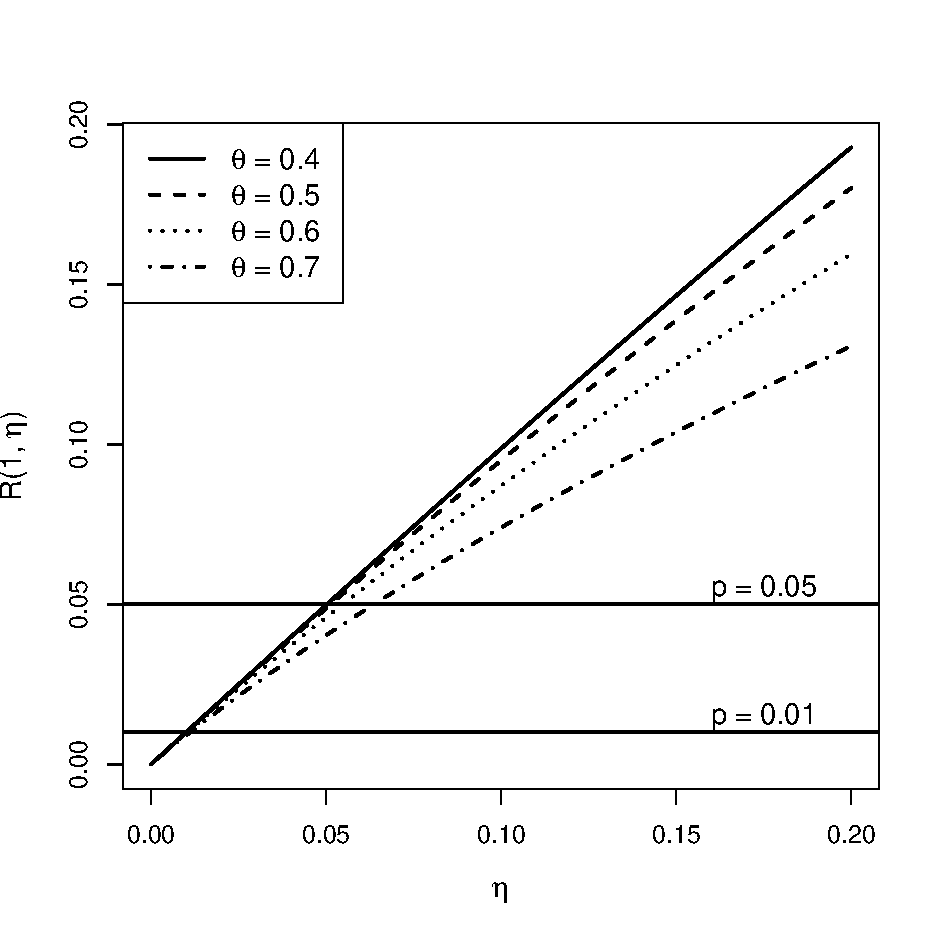
\includegraphics[width=0.3\linewidth]{tailfun_log.pdf}}
  \subfigure[H\"{u}sler-Reiss]{
    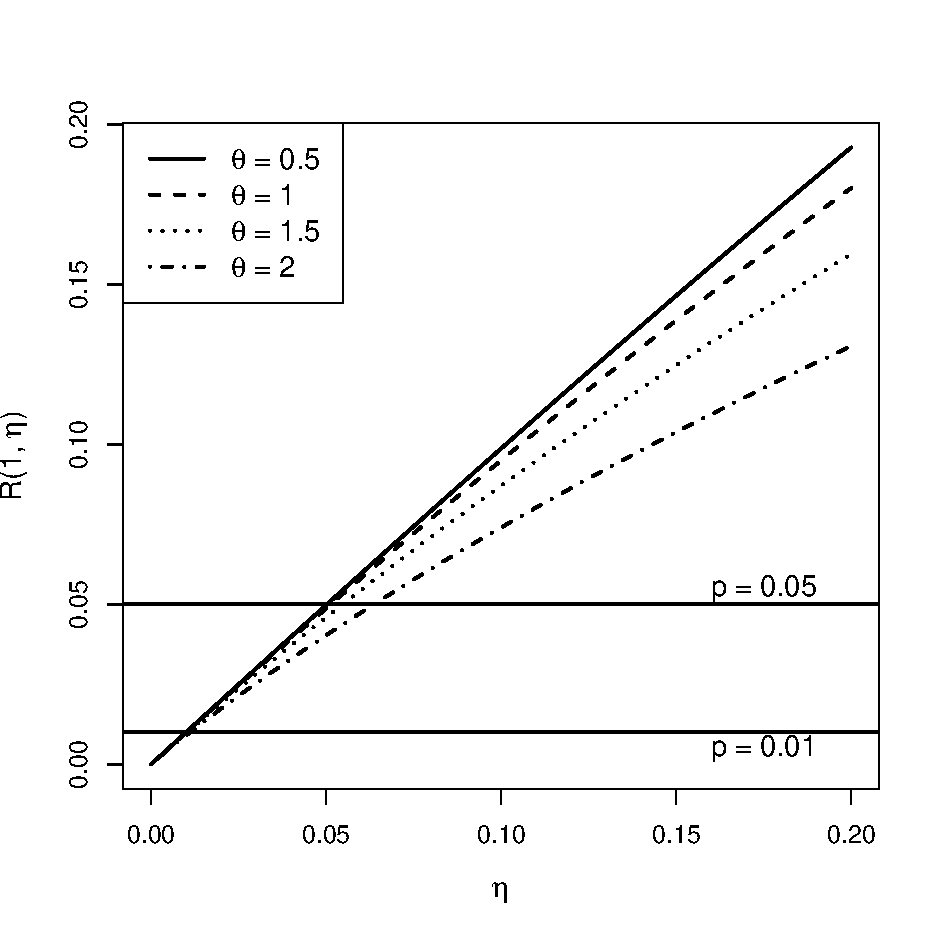
\includegraphics[width=0.3\linewidth]{tailfun_hr.pdf}}
    \subfigure[Asymmetric logistic]{
    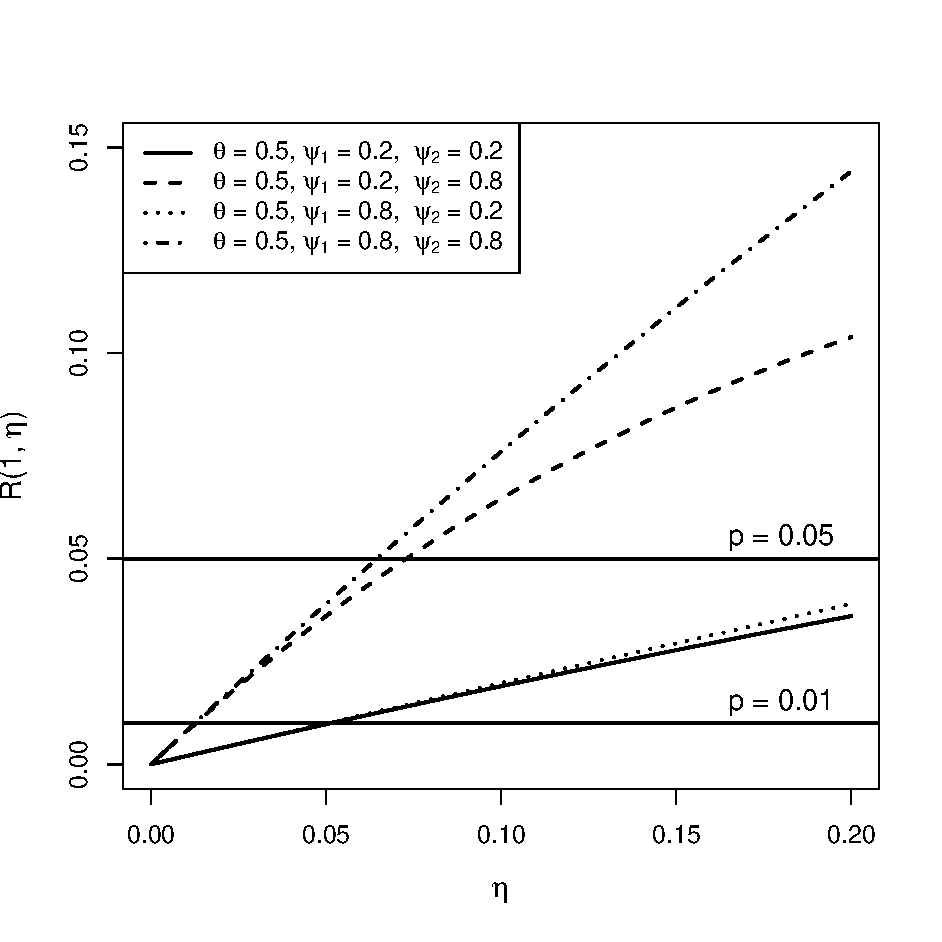
\includegraphics[width=0.3\linewidth]{tailfun_alog.pdf}}
    \subfigure[Bivariate t]{
    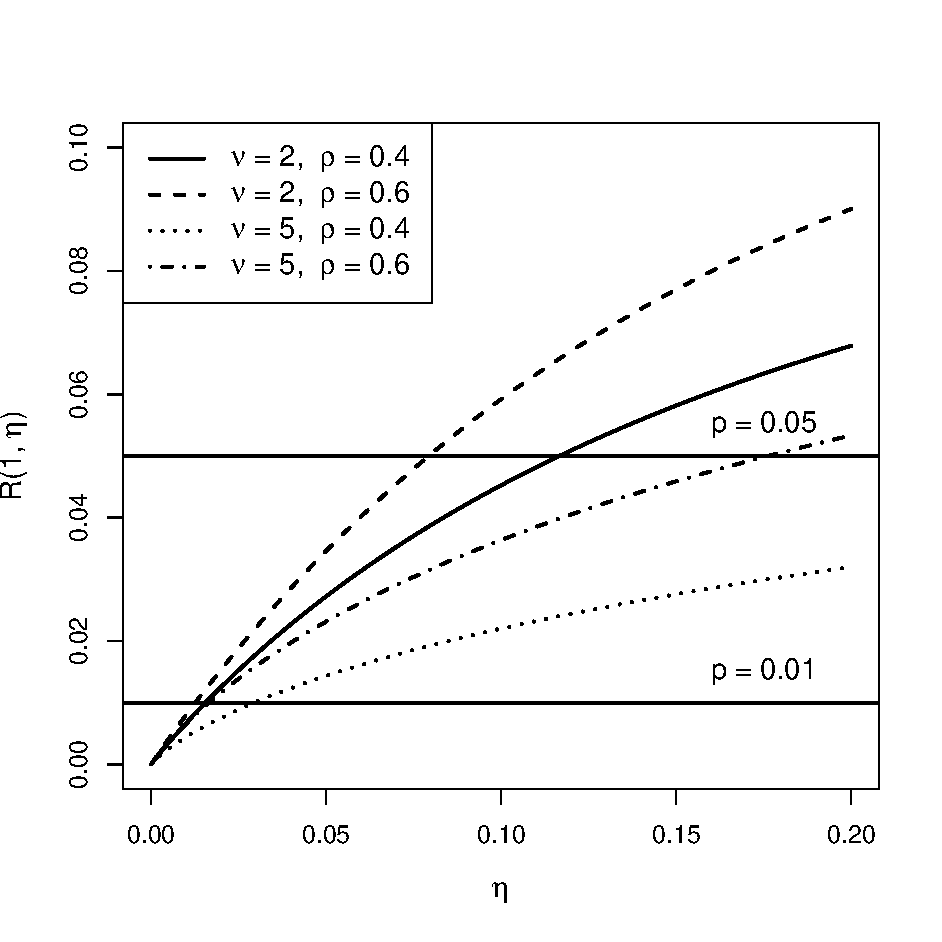
\includegraphics[width=0.3\linewidth]{tailfun_t.pdf}}
    \caption{Plots of $R(1,\eta)$ as a function of $\eta$ under various tail dependence models.}
  \label{tail_fun}
\end{figure}

\clearpage

\section{Two-stage procedure for estimating \texorpdfstring{$\CoVaR_{t}^{s|i}(p_2|p_1)$}{CoVaRt}}\label{sS4}

To estimate CoVaR dynamically, we need to apply a two-stage procedure, which can be summarized in the steps below.

\noindent{\bf Step 1 }(Univariate GARCH model estimation): Assume that $\{X_t^i\}_{t\in \nbb}$ and $\{X_t^s\}_{t\in \nbb}$ each follows an AR(1)-GARCH(1,1) process \citep{Bollerslev1986} satisfying the following model equations:
\begin{align*}
&X_t^{i} = \mu_t^{i} + \sigma_t^{i}Z_t^{i}, \quad \mu_t^{i} = \alpha_0^{i} + \alpha_1^{i}X_{t-1}^{i}, \quad (\sigma_t^{i})^2 = \beta_0^{i} + \beta_1^{i}(\sigma_{t-1}^{i}Z_{t-1}^{i})^2 + \beta_2^{i}(\sigma_{t-1}^{i})^2,\\
&X_t^{s} = \mu_t^{s} + \sigma_t^{s}Z_t^{s}, \quad \mu_t^{s} = \alpha_0^{s} + \alpha_1^{s}X_{t-1}^{s}, \quad (\sigma_t^{s})^2 = \beta_0^{s} + \beta_1^{s}(\sigma_{t-1}^{s}Z_{t-1}^{s})^2 + \beta_2^{s}(\sigma_{t-1}^{s})^2,
\end{align*}
where sequences of innovations $\{Z_t^{i}\}_{t\in \nbb}$ and $\{Z_t^{s}\}_{t\in \nbb}$ are  i.i.d. with zero mean and unit variance. Parameters of the AR(1)-GARCH(1,1) filters are estimated using maximum likelihood assuming a standardized skew-$t$ distribution (\cite{FernandezSteel1998}) for the innovations. With the estimates of conditional means and volatilities, we can obtain two sequences that could be used as proxies for realized innovations: 
\begin{equation}
\label{inno}
    \bigl\{\hat{Z}_t^{i} = (X_t^{i} - \hat{\mu}_t^{i})/{\hat{\sigma}_t^{i}}\bigr\},\qquad \bigl\{\hat{Z}_t^{s} = (X_t^{s} - \hat{\mu}_t^{s})/{\hat{\sigma}_t^{s}}\bigr\}.
\end{equation}

\noindent{\bf Step 2 }(Dynamic CoVaR estimation): Based on the time series representation of losses, $\CoVaR_{t}^{s|i}(p_2|p_1)$ can be expressed as
\begin{align*}
1 - p_2  &= \pbb\bigl(X_t^s \geq \CoVaR_{t}^{s|i}(p_2|p_1) | X_t^i\geq \VaR^i_{t}(p_1);\ \FC_{t-1}^i,\   \FC_{t-1}^s\bigr)\\
&=\pbb\Bigg(Z_t^s \geq \dfrac{\CoVaR_{t}^{s|i}(p_2|p_1)-\m_t^s}{\s_t^s}\Big | Z_t^i\geq \dfrac{\VaR^i_{t}(p_1)-\m_t^i}{\s_t^i};\ \FC_{t-1}^i,\   \FC_{t-1}^s\Biggr).
\end{align*}
This suggests first estimating risk measures based on the samples of realized innovations in \eqref{inno}, treated as i.i.d., and then computing the dynamic forecasts for time $t$ via
\begin{equation}
\widehat{\CoVaR}_{t}^{s|i}(p_2|p_1) = \hat{\mu}_t^{s} + \hat{\s}_t^s \widehat{\CoVaR}_{Z^s|Z^i}(p_2|p_1),\qquad \widehat{\VaR}^i_{t}(p_1)=\hat{\mu}_t^i + \hat{\s}_t^i\widehat{\VaR}_{Z^i}(p_1).
\end{equation}

The two-step procedure is theoretically justified as follows. First, as shown in \cite{Hoga2019_sup} (Proposition 2 in Appendix A), under the assumption that the estimation model is correctly specified, the tail empirical process based on the estimated innovations is arbitrarily close to that based on the true innovations. The difference is so small that it does not interfere with the asymptotic behavior of the latter process. This result holds for both series. Second, the results above immediately lead to the conclusion that the bivariate tail empirical process based on the two estimated innovations is arbitrarily close to that based on the two true innovations, because the difference is bounded by the sum of the differences in the two marginals. This is an obvious result due to the fact that two indicators of a joint event based on the estimated and true innovation can differ only if at least one pair of marginal indicators differs. In other words, we can show that the bivariate tail empirical process based on the two estimated innovations share the same asymptotic behavior as that based on two true innovations, which has
a bivariate Gaussian process as the limit. Such a result is the starting point for proving the asymptotic behavior of the moment estimator as in \cite{Einmahl_etal2012_sup}. Therefore, in the third step, following the lines of the proof in \cite{Einmahl_etal2012_sup}, we obtain the same asymptotic result for the moment estimator with the same speed of convergence. Fourth, we can get the asymptotic behavior of all other components needed in the proof of Theorem \ref{main_theorem_asymptotic_normality} following from the marginal tail empirical process results. Finally, combining all components and again following the proof of Theorem \ref{main_theorem_asymptotic_normality}, one can show the asymptotic normality of the estimator for the time varying CoVaR.

This strategy of proof follows similar ideas for other estimators in the literature. For instance, \cite{Hoga2022} provides an extension to situations where filtering is based on a general location-scale model. See also \cite{Girard_etal2021} for results on residual-based extreme value estimators in heavy-tailed regression models.


We note that in Step~1 above, if there is evidence of time changing correlation structure in the data, an alternative is to use a bivariate GARCH filter as was previously done in \cite{Girardi2013_sup} and \cite{NoldeZhang2018_sup}. For the data considered here, filtering out correlation led to weaker tail dependence potentially invalidating the assumption of tail dependence (for example, see Figure~\ref{sc_dcc}). We, therefore, chose to apply the GARCH filters only marginally.  

\begin{figure}[ht]
  \centering
  \subfigure{
  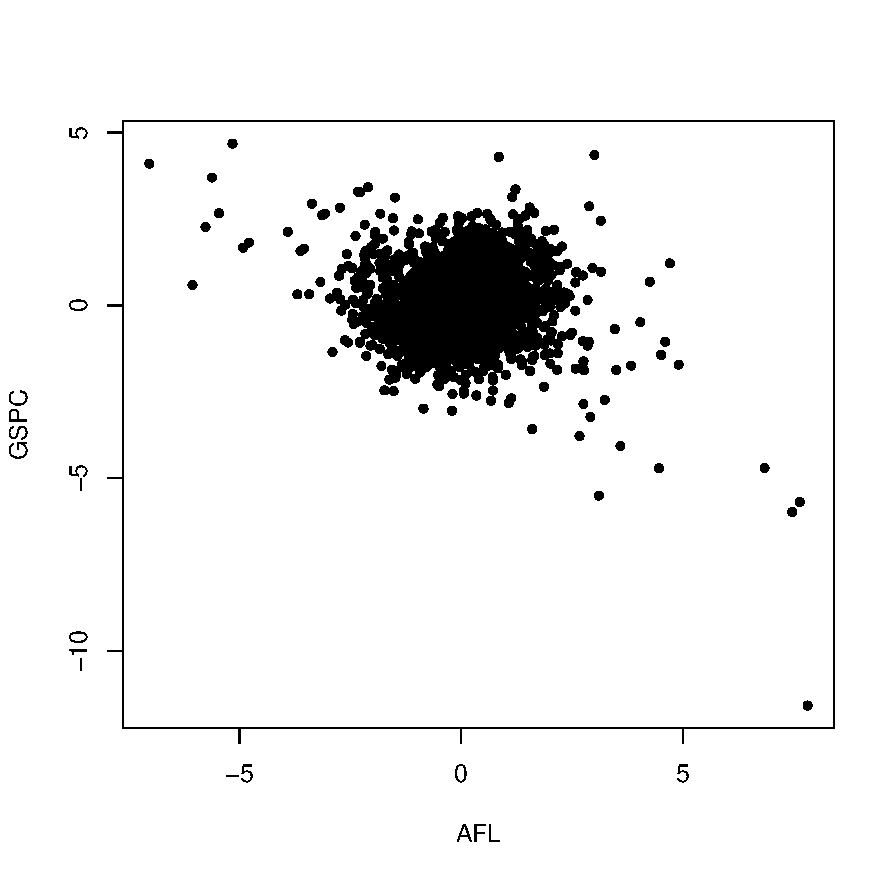
\includegraphics[width=0.4\linewidth]{scplot_AFL.pdf}}
  \subfigure{
  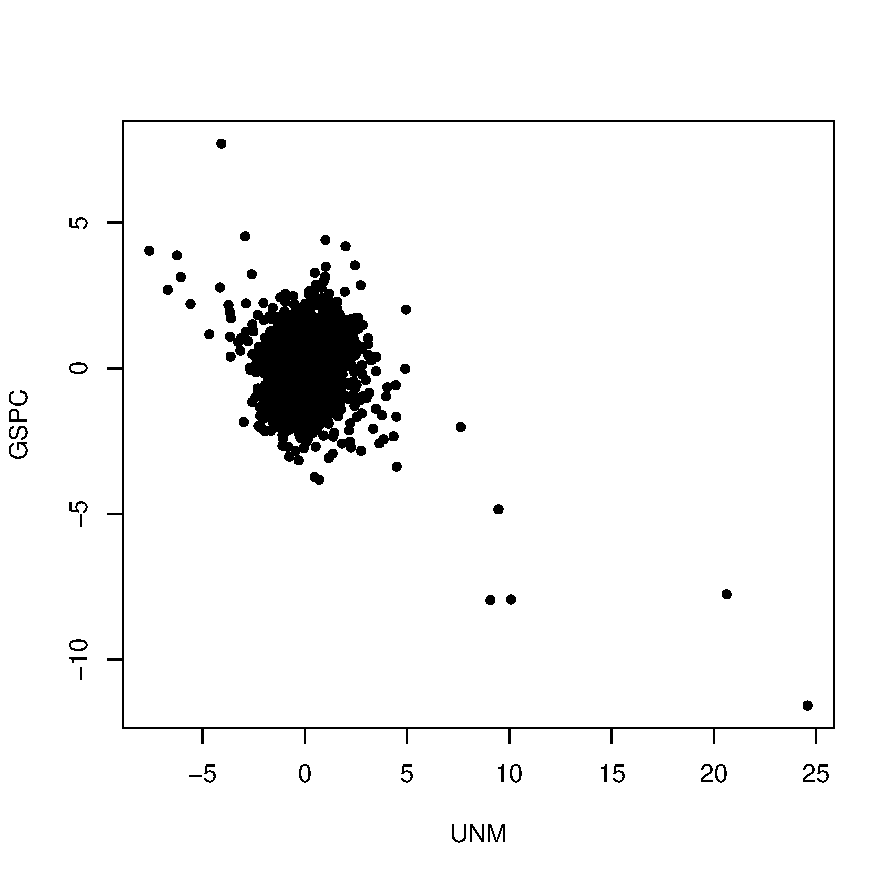
\includegraphics[width=0.4\linewidth]{scplot_UNM.pdf}}
\caption{Scatterplots of standardized innovation vectors from GARCH-DCC model for institutions AFLAC INC (AFL) and UNUMPROVIDENT CORP (UNM) with the S\&P 500 index (GSPC) as a system proxy.}
  \label{sc_dcc}
\end{figure}


\clearpage


\begin{landscape}
\section{Unconditional coverage test}
\label{uncon}

\begin{table}[H]
\tiny
\centering
\caption{Unconditional coverage tests for VaR of institutions and CoVaR at level $\pb = (0.02,0.05)$. Tail dependence models include logistic (Log),  H\"{u}sler-Reiss (HR), bilogistic (Bilog), asymmetric logistic (Alog) and that of the bivariate t distribution (t); see Supplementary Appendix~\ref{sS3} for model specifications. $E_n/e_n$ denotes the observed/nominal number of exceedances of the VaR estimate, and $E_n^b/e_n^b$ is the observed/nominal number of joint exceedances of VaR and CoVaR estimates.}
\vspace{12pt}
\begin{tabular}{cc|cccccccccccccc}
\hline
                        &           & AFL    & AIG    & ALL             & BAC             & C      & CMA    & HUM         & JPM    & LNC             & PGR    & SLM    & TRV    & UNM    & WFC    \\ \hline
\multirow{3}{*}{VaR}    & $E_n$     & 56     & 43     & 57              & 42              & 55     & 62     & 46          & 51     & 66              & 58     & 43     & 56     & 57     & 58     \\ 
                        & $e_n$     & 50.68  & 50.68  & 50.68           & 50.68           & 50.68  & 50.68  & 50.68       & 50.68  & 50.68           & 50.68  & 50.68  & 50.68  & 50.68  & 50.68  \\
                        & $p$-value & 0.4578 & 0.2633 & 0.3792          & 0.2045          & 0.5453 & 0.1205 & 0.5         & 0.9638 & \textbf{0.0377} & 0.3098 & 0.2633 & 0.4578 & 0.3792 & 0.3098 \\ \hline
\multirow{3}{*}{Log}    & $E_n^b$   & 2      & 2      & 3               & 1               & 2      & 2      & 3           & 2      & 2               & 3      & 1      & 3      & 1      & 2      \\
                        & $e_n^b$   & 2.8    & 2.15   & 2.85            & 2.1             & 2.75   & 3.1    & 2.3         & 2.55   & 3.3             & 2.9    & 2.15   & 2.8    & 2.85   & 2.9    \\
                        & $p$-value & 0.606  & 0.9155 & 0.928           & 0.3877          & 0.6265 & 0.4942 & 0.6503      & 0.7139 & 0.4297          & 0.9522 & 0.3708 & 0.9035 & 0.1965 & 0.5666 \\ \hline
\multirow{3}{*}{HR}     & $E_n^b$   & 2      & 2      & 3               & 1               & 2      & 2      & 0           & 2      & 2               & 3      & 1      & 3      & 1      & 2      \\
                        & $e_n^b$   & 2.8    & 2.15   & 2.85            & 2.1             & 2.75   & 3.1    & 2.3         & 2.55   & 3.3             & 2.9    & 2.15   & 2.8    & 2.85   & 2.9    \\
                        & $p$-value & 0.606  & 0.9155 & 0.928           & 0.3877          & 0.6265 & 0.4942 & \textbf{NA} & 0.7139 & 0.4297          & 0.9522 & 0.3708 & 0.9035 & 0.1965 & 0.5666 \\ \hline
\multirow{3}{*}{Bilog}  & $E_n^b$   & 2      & 2      & 3               & 1               & 2      & 2      & 3           & 2      & 2               & 3      & 1      & 3      & 1      & 2      \\
                        & $e_n^b$   & 2.8    & 2.15   & 2.85            & 2.1             & 2.75   & 3.1    & 2.3         & 2.55   & 3.3             & 2.9    & 2.15   & 2.8    & 2.85   & 2.9    \\
                        & $p$-value & 0.606  & 0.9155 & 0.928           & 0.3877          & 0.6265 & 0.4942 & 0.6503      & 0.7139 & 0.4297          & 0.9522 & 0.3708 & 0.9035 & 0.1965 & 0.5666 \\ \hline
\multirow{3}{*}{Alog}   & $E_n^b$   & 3      & 3      & 4               & 2               & 3      & 4      & 3           & 3      & 2               & 3      & 3      & 4      & 2      & 2      \\
                        & $e_n^b$   & 2.8    & 2.15   & 2.85            & 2.1             & 2.75   & 3.1    & 2.3         & 2.55   & 3.3             & 2.9    & 2.15   & 2.8    & 2.85   & 2.9    \\
                        & $p$-value & 0.9035 & 0.5736 & 0.5089          & 0.9431          & 0.8788 & 0.615  & 0.6503      & 0.7782 & 0.4297          & 0.9522 & 0.5736 & 0.4881 & 0.586  & 0.5666 \\ \hline
\multirow{3}{*}{t}      & $E_n^b$   & 3      & 4      & 4               & 1               & 2      & 3      & 3           & 2      & 2               & 3      & 3      & 4      & 1      & 2      \\
                        & $e_n^b$   & 2.8    & 2.15   & 2.85            & 2.1             & 2.75   & 3.1    & 2.3         & 2.55   & 3.3             & 2.9    & 2.15   & 2.8    & 2.85   & 2.9    \\
                        & $p$-value & 0.9035 & 0.245  & 0.5089          & 0.3877          & 0.6265 & 0.9533 & 0.6503      & 0.7139 & 0.4297          & 0.9522 & 0.5736 & 0.4881 & 0.1965 & 0.5666 \\ \hline
\multirow{3}{*}{FP}     & $E_n^b$   & 1      & 1      & 2               & 1               & 2      & 2      & 0           & 2      & 2               & 3      & 0      & 3      & 0      & 2      \\
                        & $e_n^b$   & 2.8    & 2.15   & 2.85            & 2.1             & 2.75   & 3.1    & 2.3         & 2.55   & 3.3             & 2.9    & 2.15   & 2.8    & 2.85   & 2.9    \\
                        & $p$-value & 0.2058  & 0.3708 & 0.5860          & 0.3877  & 0.6265 & 0.4942  & \textbf{NA}      & 0.7139 & 0.4297  & 0.9522 & \textbf{NA} & 0.9035 & \textbf{NA}  & 0.5666 \\ \hline
\multirow{3}{*}{EVT-NZ} & $E_n^b$   & 4      & 4      & 7               & 6               & 6      & 6      & 4           & 7      & 7               & 4      & 2      & 5      & 6      & 5      \\
                        & $e_n^b$   & 2.8    & 2.15   & 2.85            & 2.1             & 2.75   & 3.1    & 2.3         & 2.55   & 3.3             & 2.9    & 2.15   & 2.8    & 2.85   & 2.9    \\
                        & $p$-value & 0.4881 & 0.245  & \textbf{0.0318} & \textbf{0.0227} & 0.0798 & 0.1319 & 0.2956      & \textbf{0.0174} & 0.0672          & 0.5298 & 0.9155 & 0.2221 & 0.0931 & 0.2491 \\ \hline
\end{tabular}
\label{uncon_test}
\end{table}
\end{landscape}

\clearpage

\section{Simulation studies under model misspecification}\label{sup:Sim_Model_Misspecification}

In this section, we report results on the performance of the proposed ECQ estimator under the situation when the fitted model for the tail dependence function is misspecified. We conducted simulation studies using the settings of Section~\ref{sim}, but fit just the asymmetric logistic model for data generated using the other three tail dependence models. As summary statistics in Table~\ref{sim:summary_misspec} show, interestingly, there is both a slight lower empirical bias and a lower standard deviation when data come from the logistic and HR distributions compared to the original simulation study in which the correctly specified models were fitted. For the bivariate t distribution, there is a minor increase in bias and variance but overall results are fairly similar to those under the correct model specification. In practice, the choice of the parametric family for the tail dependence function can be based on results of comparative backtests.



\begin{table}[H]
\footnotesize
\centering
\caption{Summary statistics of ECQ estimates at level $\pb=(0.05,0.05)$ for simulation studies under model misspecification. The first row gives the true value of the ECQ under each model. }
\vspace{24pt}
\begin{tabular*}{1\textwidth}{@{\extracolsep{\fill}} c|ccc}\hline\hline
       & logistic & HR       & bivariate t      \\ \hline\hline
$Q_{Y|X}(0.05|0.05)$ & 367.31 & 399.48  & 6.81 \\  
\hline
Mean  & 389.01 & 418.78  & 6.44 \\ 
Median & 377.18 & 409.95  & 6.30 \\ 
Standard deviation     & 89.34 & 84.43 &  1.20 \\ \hline
\end{tabular*}
\label{sim:summary_misspec}
\end{table}

\begin{figure}[H]
  \centering 
  \subfigure[Logistic model]{
    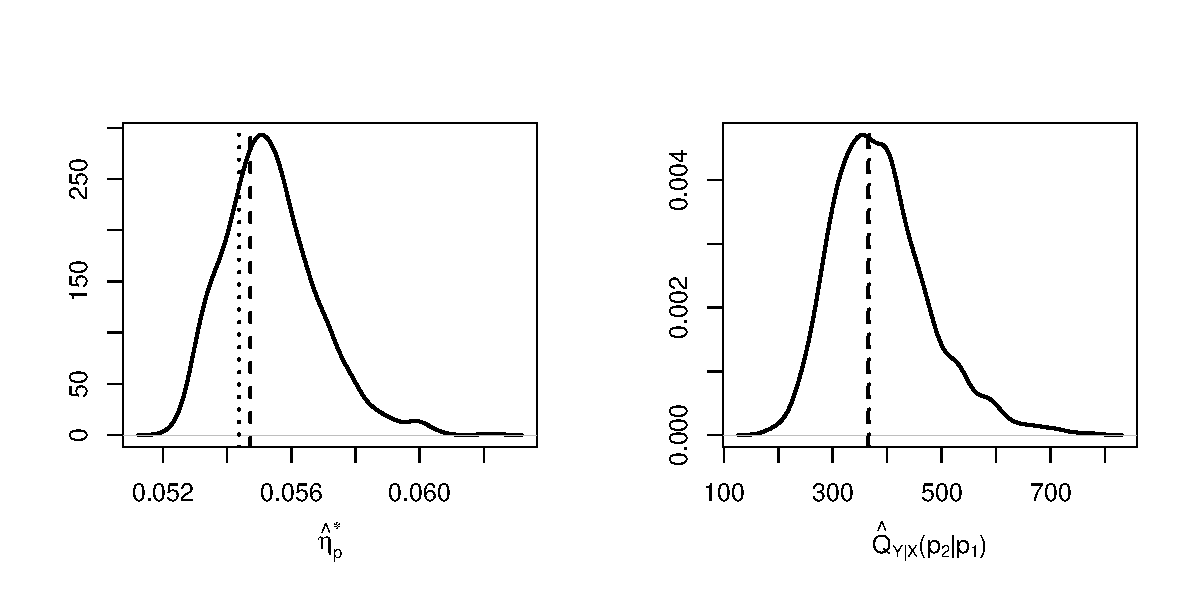
\includegraphics[width=0.6\linewidth]{log_alog.pdf}}
    \end{figure}
    \begin{figure}[H]
      \centering 
    \subfigure[HR model]{
    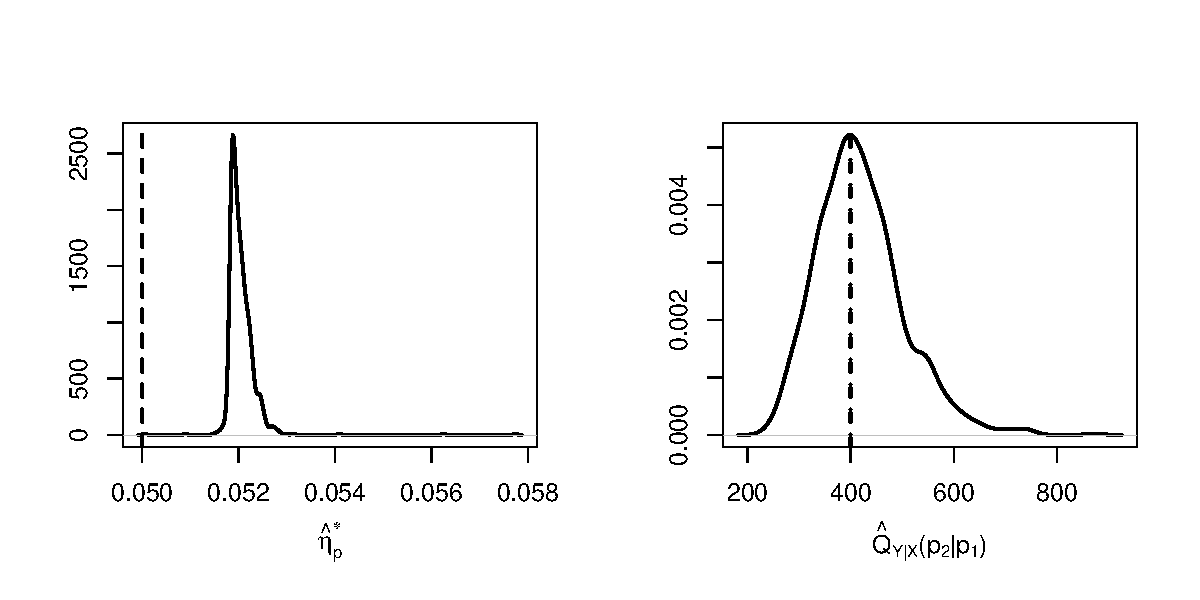
\includegraphics[width=0.6\linewidth]{hr_alog.pdf}}
    \end{figure}
    \begin{figure}[H]
          \centering 
    \subfigure[Bivariate t model]{
    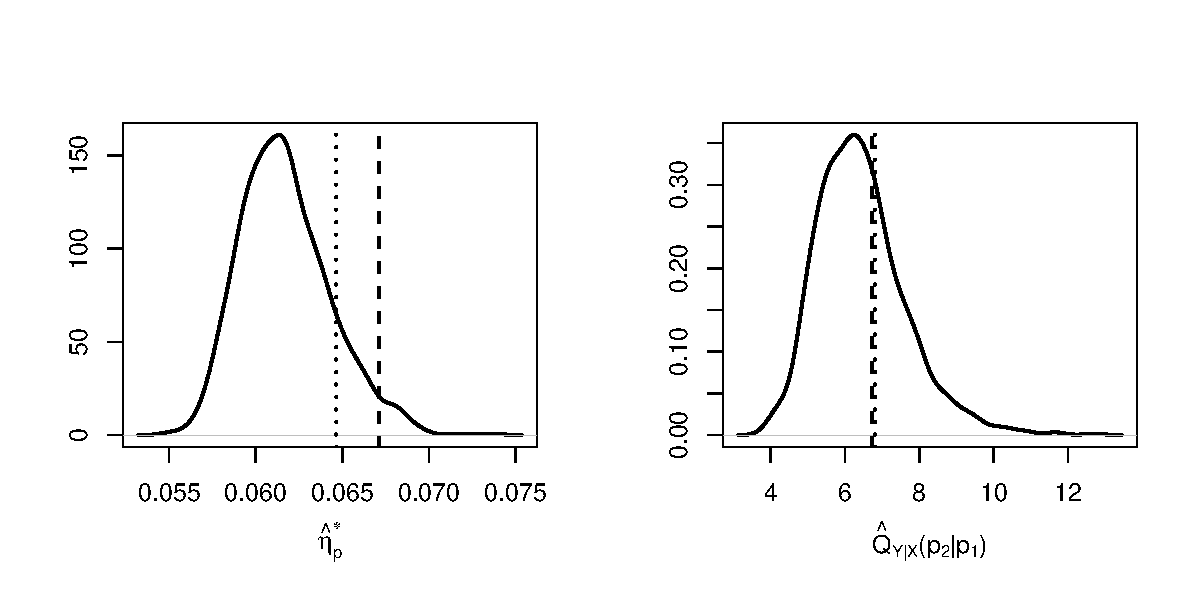
\includegraphics[width=0.6\linewidth]{t_alog.pdf}}
  \caption{The sampling densities of estimates of $\gamma$,  $\eta_p^*$, $Q_Y(p_2)$ and $Q_{Y|X}(p_2|p_1)$ for $p_1=p_2=0.05$ in the simulation study under model misspecification. The dotted vertical lines indicate true values of the quantities being estimated. The dashed vertical lines indicate the true values of $\eta_\pb$ and $Q_{Y|X}^*(p_2|p_1)$, respectively.}
  \label{sim:plot_misspec}
\end{figure}

%\clearpage

\bibliographystyle{plainnat} 

\begin{thebibliography}{29}
\providecommand{\natexlab}[1]{#1}
\providecommand{\url}[1]{\texttt{#1}}
\expandafter\ifx\csname urlstyle\endcsname\relax
  \providecommand{\doi}[1]{doi: #1}\else
  \providecommand{\doi}{doi: \begingroup \urlstyle{rm}\Url}\fi
  
\bibitem[Bollerslev(1986)]{Bollerslev1986}
T.~Bollerslev.
\newblock Generalized autoregressive conditional heteroskedasticity.
\newblock \emph{Journal of Econometrics}, 31:\penalty0 307--327, 1986.  
  
%\bibitem[de~Haan and Ferreira(2006)]{dHF2006_sup}
%L.~de~Haan and A.~Ferreira.
%\newblock \emph{Extreme Value Theory: An Introduction}.
%\newblock Springer Science \& Business Media, 2006.

\bibitem[Demarta and McNeil(2005)]{DemartaMcNeil2005}
S. Demarta and A.~J. McNeil.
\newblock The t copula and related copulas.
\newblock \emph{International Statistical Review}, 73\penalty0:\penalty0
  111--129, 2005.

%\bibitem[Einmahl et~al.(2012)Einmahl, Krajina, and Segers]{Einmahl_etal2012_sup}
%J.H. Einmahl, A.~Krajina, and J.~Segers.
%\newblock An {M}-estimator for tail dependence in arbitrary dimensions.
%\newblock \emph{The Annals of Statistics}, 40:\penalty0 1764--1793, 2012.
  
\bibitem[Fern{\'a}ndez and Steel(1998)]{FernandezSteel1998}
C.~Fern{\'a}ndez and M.~Steel.
\newblock On {B}ayesian modeling of fat tails and skewness.
\newblock \emph{Journal of the American Statistical Association}, 93:\penalty0
  359--371, 1998.
  
\bibitem[Girard et~al.(2021)Girard, Stupfler and Usseglio-Carleve]{Girard_etal2021}
S. Girard, G. Stupfler and A. Usseglio-Carleve.
\newblock Extreme conditional expectile estimation in heavy-tailed heteroscedastic regression models.
\newblock \emph{Annals of Statistics}, 49(6):\penalty0 3358–3382, 2021.

    
  
\bibitem[Girardi and Erg{\"u}n(2013)]{Girardi2013_sup}
G.~Girardi and A.T. Erg{\"u}n.
\newblock Systemic risk measurement: Multivariate {GARCH} estimation of
  {CoVaR}.
\newblock \emph{Journal of Banking \& Finance}, 37:\penalty0 3169--3180, 2013.

\bibitem[Hoga(2019)]{Hoga2019_sup}
Y. Hoga.
\newblock Confidence intervals for conditional tail risk measures in ARMA--GARCH models.
\newblock \emph{Journal of Business \& Economic Statistics}, 37(4): 613--624, 2019.

\bibitem[Hoga(2022)]{Hoga2022}
Y. Hoga.
\newblock Limit theory for forecasts of extreme distortion risk measures and expectiles.
\newblock \emph{Journal of Financial Econometrics}, 20(1): 18–44, 2022.


\bibitem[Nolde and Zhang(2020)]{NoldeZhang2018_sup}
N.~Nolde and J.~Zhang.
\newblock Conditional extremes in asymmetric financial markets.
\newblock \emph{Journal of Business \& Economic Statistics}, 38: 201--213, 2020.

\end{thebibliography}

%\end{appendices}


\end{document}
